\documentclass[../zhang_thesis.tex]{subfiles}
\begin{document}

\chapter{Filtering Results}

%%%%%%%%%%%%%%%%%%%%%%%%%%%%%%%%%%%%%%%%%%%%%%%%%%%%%%%%%%%%%%%

\section{Performance Measures}

The study was concerned with the accuracy and speed of the nonlinear filters on estimation of the SOC $x_1$. The accuracy was measured using the mean RMSE (MRMSE). The RMSE is defined as
\begin{equation}
    \mathrm{RMSE}(kT_s) = \sqrt{ \frac{1}{N_\text{trials}} \sum_{j=1}^{N_\text{trials}} \Big( \hat{x}_1^{(j)}(kT_s) - x_1^{(j)}(kT_s) \Big)^2 },
\end{equation}
where $T_s$ is the sample period and the superscript $j$ indicates the $j$th Monte Carlo trial. This study used $N_\text{trials}=100$ Monte Carlo trials. Then, the MRMSE is the mean of the RMSE over time, giving
\begin{equation}
    \mathrm{MRMSE} = \frac{1}{N} \sum_{k=1}^N \mathrm{RMSE}(kT_s),
\end{equation}
where $N$ is the total number of times at which the filtering was performed. An additional measure of accuracy was the number of trials in which the filter estimate diverged. A divergence is considered an absolute error in teh estimated SOC greater than $0.1$~V or any failure in the filtering process, such as due to a non-invertible matrix or a non-positive definite covariance matrix. In addition, after a numerical failure for a filter in a trial, no attempt was made to keep filtering the
system, and the remainder of the SOC values are assumed to be the worst case of zero. The speed was measured using the CPU time, which is the sum of the times used by the filter program on each of the CPU cores. The use of the CPU time results in less variability between runs compared to the clock time. In addition, the time taken to read and write the data is not counted.

The remainder of this chapter shows the filtering results for sampling periods of $T_s=30$, 150, and 300 seconds. Additionally, integration steps of $M=1,2,4,\dots,256$ were used for each sampling period.

\clearpage

\section{Sampling Period of 30 Seconds}

From \cref{tab:div_30}, it can be seen that the filters have no divergences for $M=4,\dots,64$. For small $M$, all filters diverge, as expected. However, the UKF and the CKF3 also diverge for large $M$, which can be explained by numerical problems arising from the large number of integration steps. The times shown in \cref{tab:time_30} show that the EKF is the fastest by far, about three to four times the speed of the next fastest, the SLF. Additionally, the EKF is about five times the speed of the UKF and the CKF3 and more than twelve times the speed of the CKF5. 

\begin{table}[h]
\centering
\caption{Number of divergences in 100 Monte Carlo runs for $T_s=30$~s as a function of number of integration steps $M$}
\begin{tabular}{@{}l*{9}{c}@{}}
\toprule
Filter/$M$ & 1   & 2   & 4 & 8 & 16 & 32 & 64 & 128 & 256 \\
\midrule
EKF        & 88  & 56  & 0 & 0 & 0  & 0 & 0 & 0 & 0   \\
UKF        & 91  & 8   & 0 & 0 & 0  & 0 & 0 & 3 & 26  \\
CKF3       & 96  & 6   & 0 & 0 & 0  & 0 & 0 & 0 & 1   \\
CKF5       & 100 & 95  & 0 & 0 & 0  & 0 & 0 & 0 & 0   \\
SLF        & 100 & 100 & 0 & 0 & 0  & 0 & 0 & 0 & 0   \\
\bottomrule
\end{tabular}
\label{tab:div_30}
\end{table}

\begin{table}[h]
\centering
\caption{Filtering time in seconds for 100 Monte Carlo runs for $T_s=30$~s as a function of number of integration steps $M$}
\begin{tabular}{@{}lccccccccc@{}}
\toprule
Filter/$M$ & 1     & 2     & 4     & 8     & 16    & 32    & 64    & 128   & 256   \\ \midrule
EKF        & 4.253 & 5.017 & 4.951 & 9.708 & 19.32 & 38.8  & 77.11 & 154   & 307.9 \\
UKF        & 4.834 & 11.85 & 23.65 & 47.24 & 93.46 & 186.5 & 373.1 & 732.9 & 1274  \\
CKF3       & 4.221 & 10.61 & 21.1  & 41.33 & 82.57 & 165   & 328.2 & 657.9 & 1317  \\
CKF5       & 9.533 & 28.82 & 59.49 & 117.8 & 234.9 & 468.8 & 937.9 & 1873  & 3748  \\
SLF        & 4.521 & 6.52  & 16.35 & 32.11 & 63.43 & 126.7 & 252.1 & 503.5 & 1006  \\ \bottomrule
\end{tabular}
\label{tab:time_30}
\end{table}

\cref{fig:mrmse_30} shows the MRMSE as a function of the number of integration steps over the divergence-free range. It can be see that the EKF result shows a decrease over this range as expected. However, the other results have minimum error at $M=16$, with an increase in error for larger $M$. This could be due to numerical errors that also caused divergences for large $M$ in the case of the UKF and the CKF3. The global minimum error is given by both the CKF5 and the SLF at $M=16$. For comparison purposes, the RMSE at $M=4$ and 64 are shown in \cref{fig:rmse_30_4,fig:rmse_30_64}. The RMSEs for the filters are all very close in value, as expected from the closeness of the MRMSE values. It can be seen that the RMSEs increase during the period of high-rate charge and discharge, when the nonlinear effects are the strongest. These increases are less pronounced for $M=64$ than for $M=4$, as expected. The fluctuations in the RMSE occur when transitioning between charging and discharging.

\begin{figure}[b]
\centering
% This file is generated by the MATLAB m-file laprint.m. It can be included
% into LaTeX documents using the packages graphicx, color and psfrag.
% It is accompanied by a postscript file. A sample LaTeX file is:
%    \documentclass{article}\usepackage{graphicx,color,psfrag}
%    \begin{document}% This file is generated by the MATLAB m-file laprint.m. It can be included
% into LaTeX documents using the packages graphicx, color and psfrag.
% It is accompanied by a postscript file. A sample LaTeX file is:
%    \documentclass{article}\usepackage{graphicx,color,psfrag}
%    \begin{document}% This file is generated by the MATLAB m-file laprint.m. It can be included
% into LaTeX documents using the packages graphicx, color and psfrag.
% It is accompanied by a postscript file. A sample LaTeX file is:
%    \documentclass{article}\usepackage{graphicx,color,psfrag}
%    \begin{document}\input{mrmse_30}\end{document}
% See http://www.mathworks.de/matlabcentral/fileexchange/loadFile.do?objectId=4638
% for recent versions of laprint.m.
%
% created by:           LaPrint version 3.16 (13.9.2004)
% created on:           22-Apr-2014 12:33:29
% eps bounding box:     15 cm x 11.0893 cm
% comment:              
%
\begin{psfrags}%
\psfragscanon%
%
% text strings:
\psfrag{s01}[t][t]{\color[rgb]{0,0,0}\setlength{\tabcolsep}{0pt}\begin{tabular}{c}$\log_2 (M)$\end{tabular}}%
\psfrag{s02}[b][b]{\color[rgb]{0,0,0}\setlength{\tabcolsep}{0pt}\begin{tabular}{c}MRMSE\end{tabular}}%
\psfrag{s06}[][]{\color[rgb]{0,0,0}\setlength{\tabcolsep}{0pt}\begin{tabular}{c} \end{tabular}}%
\psfrag{s07}[][]{\color[rgb]{0,0,0}\setlength{\tabcolsep}{0pt}\begin{tabular}{c} \end{tabular}}%
\psfrag{s08}[l][l]{\color[rgb]{0,0,0}SLF}%
\psfrag{s13}[l][l]{\color[rgb]{0,0,0}EKF}%
\psfrag{s14}[l][l]{\color[rgb]{0,0,0}UKF}%
\psfrag{s15}[l][l]{\color[rgb]{0,0,0}CKF3}%
\psfrag{s16}[l][l]{\color[rgb]{0,0,0}CKF5}%
\psfrag{s17}[l][l]{\color[rgb]{0,0,0}SLF}%
%
% xticklabels:
\psfrag{x01}[t][t]{0}%
\psfrag{x02}[t][t]{0.1}%
\psfrag{x03}[t][t]{0.2}%
\psfrag{x04}[t][t]{0.3}%
\psfrag{x05}[t][t]{0.4}%
\psfrag{x06}[t][t]{0.5}%
\psfrag{x07}[t][t]{0.6}%
\psfrag{x08}[t][t]{0.7}%
\psfrag{x09}[t][t]{0.8}%
\psfrag{x10}[t][t]{0.9}%
\psfrag{x11}[t][t]{1}%
\psfrag{x12}[t][t]{2}%
\psfrag{x13}[t][t]{3}%
\psfrag{x14}[t][t]{4}%
\psfrag{x15}[t][t]{5}%
\psfrag{x16}[t][t]{6}%
%
% yticklabels:
\psfrag{v01}[r][r]{0}%
\psfrag{v02}[r][r]{0.1}%
\psfrag{v03}[r][r]{0.2}%
\psfrag{v04}[r][r]{0.3}%
\psfrag{v05}[r][r]{0.4}%
\psfrag{v06}[r][r]{0.5}%
\psfrag{v07}[r][r]{0.6}%
\psfrag{v08}[r][r]{0.7}%
\psfrag{v09}[r][r]{0.8}%
\psfrag{v10}[r][r]{0.9}%
\psfrag{v11}[r][r]{1}%
\psfrag{v12}[r][r]{4.5}%
\psfrag{v13}[r][r]{5}%
\psfrag{v14}[r][r]{5.5}%
\psfrag{v15}[r][r]{6}%
\psfrag{ypower3}[Bl][Bl]{$\times 10^{-3}$}%
%
% Figure:
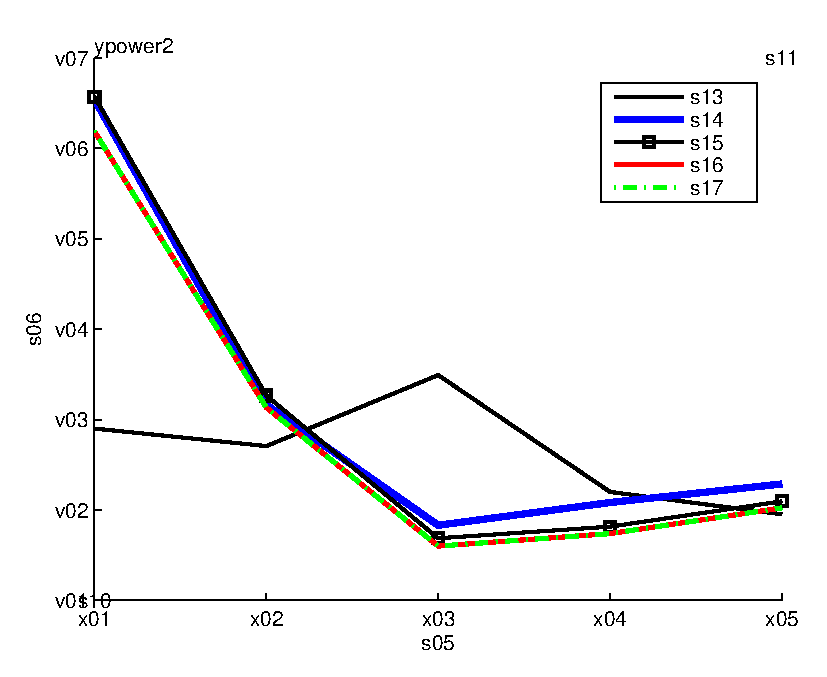
\includegraphics[width=15cm]{mrmse_30.eps}%
\end{psfrags}%
%
% End mrmse_30.tex
\end{document}
% See http://www.mathworks.de/matlabcentral/fileexchange/loadFile.do?objectId=4638
% for recent versions of laprint.m.
%
% created by:           LaPrint version 3.16 (13.9.2004)
% created on:           22-Apr-2014 12:33:29
% eps bounding box:     15 cm x 11.0893 cm
% comment:              
%
\begin{psfrags}%
\psfragscanon%
%
% text strings:
\psfrag{s01}[t][t]{\color[rgb]{0,0,0}\setlength{\tabcolsep}{0pt}\begin{tabular}{c}$\log_2 (M)$\end{tabular}}%
\psfrag{s02}[b][b]{\color[rgb]{0,0,0}\setlength{\tabcolsep}{0pt}\begin{tabular}{c}MRMSE\end{tabular}}%
\psfrag{s06}[][]{\color[rgb]{0,0,0}\setlength{\tabcolsep}{0pt}\begin{tabular}{c} \end{tabular}}%
\psfrag{s07}[][]{\color[rgb]{0,0,0}\setlength{\tabcolsep}{0pt}\begin{tabular}{c} \end{tabular}}%
\psfrag{s08}[l][l]{\color[rgb]{0,0,0}SLF}%
\psfrag{s13}[l][l]{\color[rgb]{0,0,0}EKF}%
\psfrag{s14}[l][l]{\color[rgb]{0,0,0}UKF}%
\psfrag{s15}[l][l]{\color[rgb]{0,0,0}CKF3}%
\psfrag{s16}[l][l]{\color[rgb]{0,0,0}CKF5}%
\psfrag{s17}[l][l]{\color[rgb]{0,0,0}SLF}%
%
% xticklabels:
\psfrag{x01}[t][t]{0}%
\psfrag{x02}[t][t]{0.1}%
\psfrag{x03}[t][t]{0.2}%
\psfrag{x04}[t][t]{0.3}%
\psfrag{x05}[t][t]{0.4}%
\psfrag{x06}[t][t]{0.5}%
\psfrag{x07}[t][t]{0.6}%
\psfrag{x08}[t][t]{0.7}%
\psfrag{x09}[t][t]{0.8}%
\psfrag{x10}[t][t]{0.9}%
\psfrag{x11}[t][t]{1}%
\psfrag{x12}[t][t]{2}%
\psfrag{x13}[t][t]{3}%
\psfrag{x14}[t][t]{4}%
\psfrag{x15}[t][t]{5}%
\psfrag{x16}[t][t]{6}%
%
% yticklabels:
\psfrag{v01}[r][r]{0}%
\psfrag{v02}[r][r]{0.1}%
\psfrag{v03}[r][r]{0.2}%
\psfrag{v04}[r][r]{0.3}%
\psfrag{v05}[r][r]{0.4}%
\psfrag{v06}[r][r]{0.5}%
\psfrag{v07}[r][r]{0.6}%
\psfrag{v08}[r][r]{0.7}%
\psfrag{v09}[r][r]{0.8}%
\psfrag{v10}[r][r]{0.9}%
\psfrag{v11}[r][r]{1}%
\psfrag{v12}[r][r]{4.5}%
\psfrag{v13}[r][r]{5}%
\psfrag{v14}[r][r]{5.5}%
\psfrag{v15}[r][r]{6}%
\psfrag{ypower3}[Bl][Bl]{$\times 10^{-3}$}%
%
% Figure:
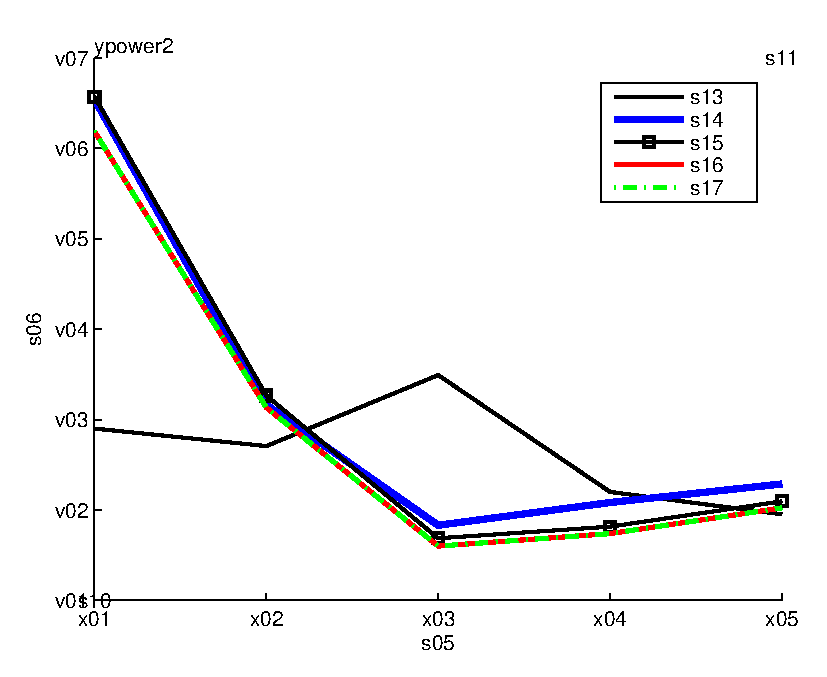
\includegraphics[width=15cm]{mrmse_30.eps}%
\end{psfrags}%
%
% End mrmse_30.tex
\end{document}
% See http://www.mathworks.de/matlabcentral/fileexchange/loadFile.do?objectId=4638
% for recent versions of laprint.m.
%
% created by:           LaPrint version 3.16 (13.9.2004)
% created on:           22-Apr-2014 12:33:29
% eps bounding box:     15 cm x 11.0893 cm
% comment:              
%
\begin{psfrags}%
\psfragscanon%
%
% text strings:
\psfrag{s01}[t][t]{\color[rgb]{0,0,0}\setlength{\tabcolsep}{0pt}\begin{tabular}{c}$\log_2 (M)$\end{tabular}}%
\psfrag{s02}[b][b]{\color[rgb]{0,0,0}\setlength{\tabcolsep}{0pt}\begin{tabular}{c}MRMSE\end{tabular}}%
\psfrag{s06}[][]{\color[rgb]{0,0,0}\setlength{\tabcolsep}{0pt}\begin{tabular}{c} \end{tabular}}%
\psfrag{s07}[][]{\color[rgb]{0,0,0}\setlength{\tabcolsep}{0pt}\begin{tabular}{c} \end{tabular}}%
\psfrag{s08}[l][l]{\color[rgb]{0,0,0}SLF}%
\psfrag{s13}[l][l]{\color[rgb]{0,0,0}EKF}%
\psfrag{s14}[l][l]{\color[rgb]{0,0,0}UKF}%
\psfrag{s15}[l][l]{\color[rgb]{0,0,0}CKF3}%
\psfrag{s16}[l][l]{\color[rgb]{0,0,0}CKF5}%
\psfrag{s17}[l][l]{\color[rgb]{0,0,0}SLF}%
%
% xticklabels:
\psfrag{x01}[t][t]{0}%
\psfrag{x02}[t][t]{0.1}%
\psfrag{x03}[t][t]{0.2}%
\psfrag{x04}[t][t]{0.3}%
\psfrag{x05}[t][t]{0.4}%
\psfrag{x06}[t][t]{0.5}%
\psfrag{x07}[t][t]{0.6}%
\psfrag{x08}[t][t]{0.7}%
\psfrag{x09}[t][t]{0.8}%
\psfrag{x10}[t][t]{0.9}%
\psfrag{x11}[t][t]{1}%
\psfrag{x12}[t][t]{2}%
\psfrag{x13}[t][t]{3}%
\psfrag{x14}[t][t]{4}%
\psfrag{x15}[t][t]{5}%
\psfrag{x16}[t][t]{6}%
%
% yticklabels:
\psfrag{v01}[r][r]{0}%
\psfrag{v02}[r][r]{0.1}%
\psfrag{v03}[r][r]{0.2}%
\psfrag{v04}[r][r]{0.3}%
\psfrag{v05}[r][r]{0.4}%
\psfrag{v06}[r][r]{0.5}%
\psfrag{v07}[r][r]{0.6}%
\psfrag{v08}[r][r]{0.7}%
\psfrag{v09}[r][r]{0.8}%
\psfrag{v10}[r][r]{0.9}%
\psfrag{v11}[r][r]{1}%
\psfrag{v12}[r][r]{4.5}%
\psfrag{v13}[r][r]{5}%
\psfrag{v14}[r][r]{5.5}%
\psfrag{v15}[r][r]{6}%
\psfrag{ypower3}[Bl][Bl]{$\times 10^{-3}$}%
%
% Figure:
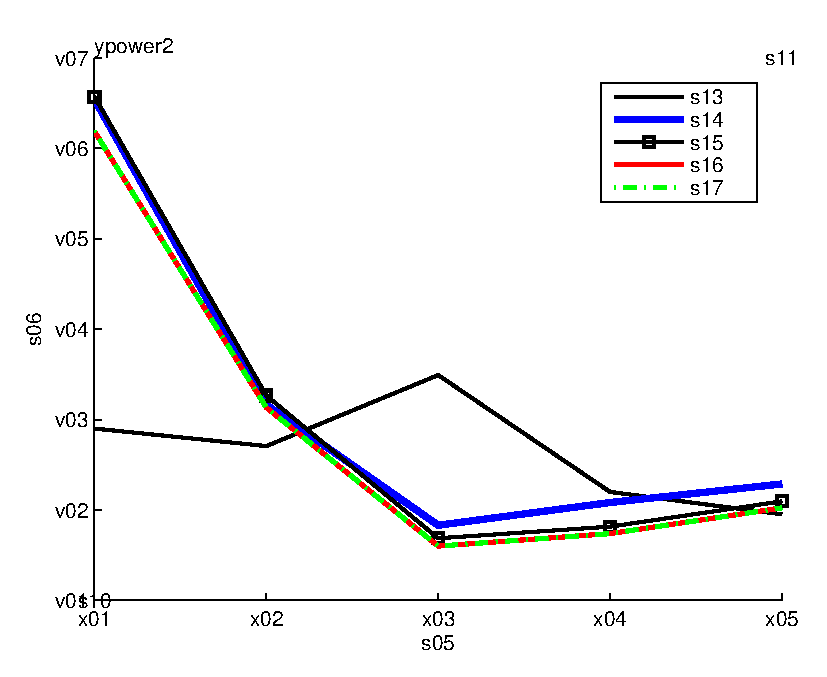
\includegraphics[width=15cm]{mrmse_30.eps}%
\end{psfrags}%
%
% End mrmse_30.tex

\caption{SOC error for $T_s=30$~s as a function of number of integration steps $M$.}
\label{fig:mrmse_30}
\end{figure}

\begin{figure}
\centering
% generated by laprint.m
%
%
% text strings:
\psfrag{s05}[b][b]{\color[rgb]{0,0,0}\setlength{\tabcolsep}{0pt}\begin{tabular}{c}RMSE\end{tabular}}%
\psfrag{s06}[t][t]{\color[rgb]{0,0,0}\setlength{\tabcolsep}{0pt}\begin{tabular}{c}$k$\end{tabular}}%
\psfrag{s10}[][]{\color[rgb]{0,0,0}\setlength{\tabcolsep}{0pt}\begin{tabular}{c} \end{tabular}}%
\psfrag{s11}[][]{\color[rgb]{0,0,0}\setlength{\tabcolsep}{0pt}\begin{tabular}{c} \end{tabular}}%
\psfrag{s12}[l][l]{\color[rgb]{0,0,0}SLF}%
\psfrag{s13}[l][l]{\color[rgb]{0,0,0}EKF}%
\psfrag{s14}[l][l]{\color[rgb]{0,0,0}UKF}%
\psfrag{s15}[l][l]{\color[rgb]{0,0,0}CKF3}%
\psfrag{s16}[l][l]{\color[rgb]{0,0,0}CKF5}%
\psfrag{s17}[l][l]{\color[rgb]{0,0,0}SLF}%
%
% xticklabels:
\psfrag{x01}[t][t]{0}%
\psfrag{x02}[t][t]{500}%
\psfrag{x03}[t][t]{1000}%
\psfrag{x04}[t][t]{1500}%
\psfrag{x05}[t][t]{2000}%
\psfrag{x06}[t][t]{2500}%
\psfrag{x07}[t][t]{3000}%
\psfrag{x08}[t][t]{3500}%
%
% yticklabels:
\psfrag{v01}[r][r]{0}%
\psfrag{v02}[r][r]{0.005}%
\psfrag{v03}[r][r]{0.01}%
\psfrag{v04}[r][r]{0.015}%
\psfrag{v05}[r][r]{0.02}%
\psfrag{v06}[r][r]{0.025}%
\psfrag{v07}[r][r]{0.03}%
\psfrag{v08}[r][r]{0.035}%
%
% Figure:
%
% End rmse_30_4.tex

\caption{RMSE of SOC estimation for $T_s=30$~s and $M=4$.}
\label{fig:rmse_30_4}
\end{figure}

\begin{figure}
\centering
% This file is generated by the MATLAB m-file laprint.m. It can be included
% into LaTeX documents using the packages graphicx, color and psfrag.
% It is accompanied by a postscript file. A sample LaTeX file is:
%    \documentclass{article}\usepackage{graphicx,color,psfrag}
%    \begin{document}% This file is generated by the MATLAB m-file laprint.m. It can be included
% into LaTeX documents using the packages graphicx, color and psfrag.
% It is accompanied by a postscript file. A sample LaTeX file is:
%    \documentclass{article}\usepackage{graphicx,color,psfrag}
%    \begin{document}% This file is generated by the MATLAB m-file laprint.m. It can be included
% into LaTeX documents using the packages graphicx, color and psfrag.
% It is accompanied by a postscript file. A sample LaTeX file is:
%    \documentclass{article}\usepackage{graphicx,color,psfrag}
%    \begin{document}\input{rmse_30_64}\end{document}
% See http://www.mathworks.de/matlabcentral/fileexchange/loadFile.do?objectId=4638
% for recent versions of laprint.m.
%
% created by:           LaPrint version 3.16 (13.9.2004)
% created on:           22-Apr-2014 13:13:51
% eps bounding box:     15 cm x 19.9821 cm
% comment:              
%
\begin{psfrags}%
\psfragscanon%
%
% text strings:
\psfrag{s14}[b][b]{\color[rgb]{0,0,0}\setlength{\tabcolsep}{0pt}\begin{tabular}{c}EKF\end{tabular}}%
\psfrag{s15}[b][b]{\color[rgb]{0,0,0}\setlength{\tabcolsep}{0pt}\begin{tabular}{c}UKF\end{tabular}}%
\psfrag{s16}[b][b]{\color[rgb]{0,0,0}\setlength{\tabcolsep}{0pt}\begin{tabular}{c}RMSE\end{tabular}}%
\psfrag{s17}[b][b]{\color[rgb]{0,0,0}\setlength{\tabcolsep}{0pt}\begin{tabular}{c}CKF3\end{tabular}}%
\psfrag{s18}[b][b]{\color[rgb]{0,0,0}\setlength{\tabcolsep}{0pt}\begin{tabular}{c}CKF5\end{tabular}}%
\psfrag{s19}[b][b]{\color[rgb]{0,0,0}\setlength{\tabcolsep}{0pt}\begin{tabular}{c}SLF\end{tabular}}%
\psfrag{s20}[t][t]{\color[rgb]{0,0,0}\setlength{\tabcolsep}{0pt}\begin{tabular}{c}$k$\end{tabular}}%
%
% xticklabels:
\psfrag{x01}[t][t]{0}%
\psfrag{x02}[t][t]{500}%
\psfrag{x03}[t][t]{1000}%
\psfrag{x04}[t][t]{1500}%
\psfrag{x05}[t][t]{2000}%
\psfrag{x06}[t][t]{2500}%
\psfrag{x07}[t][t]{3000}%
\psfrag{x08}[t][t]{3500}%
\psfrag{x09}[t][t]{0}%
\psfrag{x10}[t][t]{500}%
\psfrag{x11}[t][t]{1000}%
\psfrag{x12}[t][t]{1500}%
\psfrag{x13}[t][t]{2000}%
\psfrag{x14}[t][t]{2500}%
\psfrag{x15}[t][t]{3000}%
\psfrag{x16}[t][t]{3500}%
\psfrag{x17}[t][t]{0}%
\psfrag{x18}[t][t]{500}%
\psfrag{x19}[t][t]{1000}%
\psfrag{x20}[t][t]{1500}%
\psfrag{x21}[t][t]{2000}%
\psfrag{x22}[t][t]{2500}%
\psfrag{x23}[t][t]{3000}%
\psfrag{x24}[t][t]{3500}%
\psfrag{x25}[t][t]{0}%
\psfrag{x26}[t][t]{500}%
\psfrag{x27}[t][t]{1000}%
\psfrag{x28}[t][t]{1500}%
\psfrag{x29}[t][t]{2000}%
\psfrag{x30}[t][t]{2500}%
\psfrag{x31}[t][t]{3000}%
\psfrag{x32}[t][t]{3500}%
\psfrag{x33}[t][t]{0}%
\psfrag{x34}[t][t]{500}%
\psfrag{x35}[t][t]{1000}%
\psfrag{x36}[t][t]{1500}%
\psfrag{x37}[t][t]{2000}%
\psfrag{x38}[t][t]{2500}%
\psfrag{x39}[t][t]{3000}%
\psfrag{x40}[t][t]{3500}%
%
% yticklabels:
\psfrag{v01}[r][r]{0}%
\psfrag{v02}[r][r]{0.02}%
\psfrag{v03}[r][r]{0.04}%
\psfrag{v04}[r][r]{0}%
\psfrag{v05}[r][r]{0.02}%
\psfrag{v06}[r][r]{0.04}%
\psfrag{v07}[r][r]{0}%
\psfrag{v08}[r][r]{0.02}%
\psfrag{v09}[r][r]{0.04}%
\psfrag{v10}[r][r]{0}%
\psfrag{v11}[r][r]{0.02}%
\psfrag{v12}[r][r]{0.04}%
\psfrag{v13}[r][r]{0}%
\psfrag{v14}[r][r]{0.02}%
\psfrag{v15}[r][r]{0.04}%
%
% Figure:
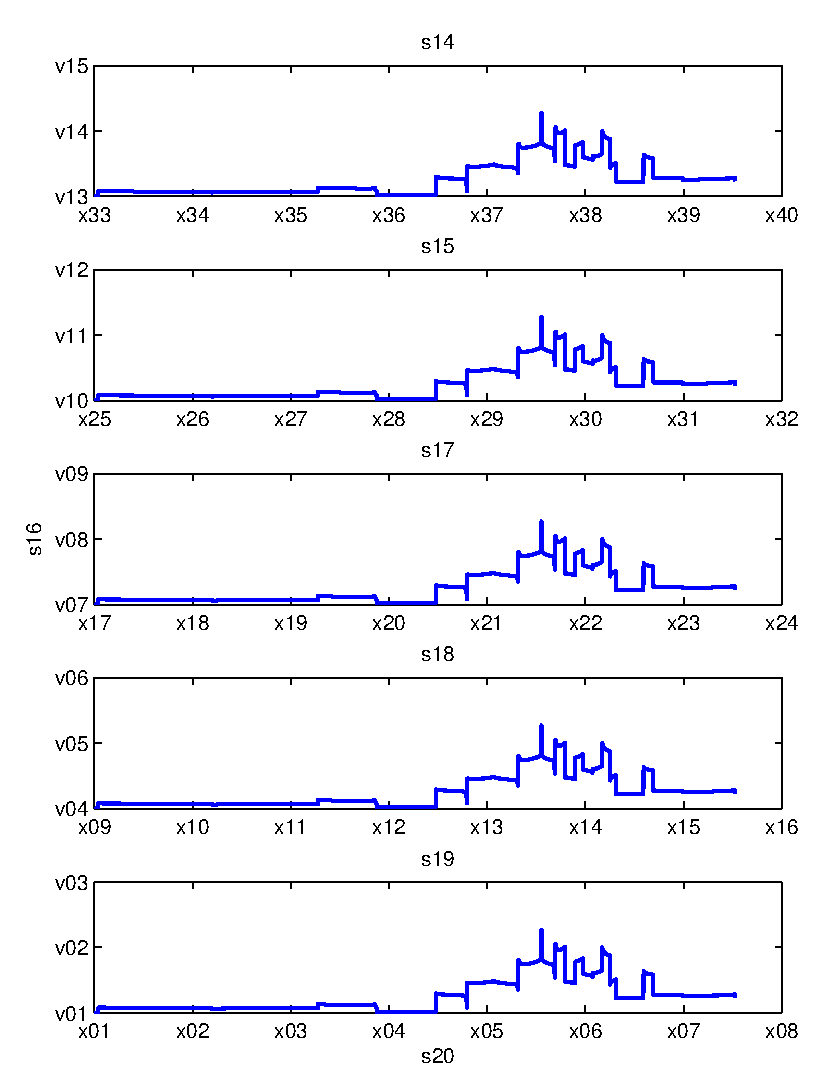
\includegraphics[width=15cm]{rmse_30_64.eps}%
\end{psfrags}%
%
% End rmse_30_64.tex
\end{document}
% See http://www.mathworks.de/matlabcentral/fileexchange/loadFile.do?objectId=4638
% for recent versions of laprint.m.
%
% created by:           LaPrint version 3.16 (13.9.2004)
% created on:           22-Apr-2014 13:13:51
% eps bounding box:     15 cm x 19.9821 cm
% comment:              
%
\begin{psfrags}%
\psfragscanon%
%
% text strings:
\psfrag{s14}[b][b]{\color[rgb]{0,0,0}\setlength{\tabcolsep}{0pt}\begin{tabular}{c}EKF\end{tabular}}%
\psfrag{s15}[b][b]{\color[rgb]{0,0,0}\setlength{\tabcolsep}{0pt}\begin{tabular}{c}UKF\end{tabular}}%
\psfrag{s16}[b][b]{\color[rgb]{0,0,0}\setlength{\tabcolsep}{0pt}\begin{tabular}{c}RMSE\end{tabular}}%
\psfrag{s17}[b][b]{\color[rgb]{0,0,0}\setlength{\tabcolsep}{0pt}\begin{tabular}{c}CKF3\end{tabular}}%
\psfrag{s18}[b][b]{\color[rgb]{0,0,0}\setlength{\tabcolsep}{0pt}\begin{tabular}{c}CKF5\end{tabular}}%
\psfrag{s19}[b][b]{\color[rgb]{0,0,0}\setlength{\tabcolsep}{0pt}\begin{tabular}{c}SLF\end{tabular}}%
\psfrag{s20}[t][t]{\color[rgb]{0,0,0}\setlength{\tabcolsep}{0pt}\begin{tabular}{c}$k$\end{tabular}}%
%
% xticklabels:
\psfrag{x01}[t][t]{0}%
\psfrag{x02}[t][t]{500}%
\psfrag{x03}[t][t]{1000}%
\psfrag{x04}[t][t]{1500}%
\psfrag{x05}[t][t]{2000}%
\psfrag{x06}[t][t]{2500}%
\psfrag{x07}[t][t]{3000}%
\psfrag{x08}[t][t]{3500}%
\psfrag{x09}[t][t]{0}%
\psfrag{x10}[t][t]{500}%
\psfrag{x11}[t][t]{1000}%
\psfrag{x12}[t][t]{1500}%
\psfrag{x13}[t][t]{2000}%
\psfrag{x14}[t][t]{2500}%
\psfrag{x15}[t][t]{3000}%
\psfrag{x16}[t][t]{3500}%
\psfrag{x17}[t][t]{0}%
\psfrag{x18}[t][t]{500}%
\psfrag{x19}[t][t]{1000}%
\psfrag{x20}[t][t]{1500}%
\psfrag{x21}[t][t]{2000}%
\psfrag{x22}[t][t]{2500}%
\psfrag{x23}[t][t]{3000}%
\psfrag{x24}[t][t]{3500}%
\psfrag{x25}[t][t]{0}%
\psfrag{x26}[t][t]{500}%
\psfrag{x27}[t][t]{1000}%
\psfrag{x28}[t][t]{1500}%
\psfrag{x29}[t][t]{2000}%
\psfrag{x30}[t][t]{2500}%
\psfrag{x31}[t][t]{3000}%
\psfrag{x32}[t][t]{3500}%
\psfrag{x33}[t][t]{0}%
\psfrag{x34}[t][t]{500}%
\psfrag{x35}[t][t]{1000}%
\psfrag{x36}[t][t]{1500}%
\psfrag{x37}[t][t]{2000}%
\psfrag{x38}[t][t]{2500}%
\psfrag{x39}[t][t]{3000}%
\psfrag{x40}[t][t]{3500}%
%
% yticklabels:
\psfrag{v01}[r][r]{0}%
\psfrag{v02}[r][r]{0.02}%
\psfrag{v03}[r][r]{0.04}%
\psfrag{v04}[r][r]{0}%
\psfrag{v05}[r][r]{0.02}%
\psfrag{v06}[r][r]{0.04}%
\psfrag{v07}[r][r]{0}%
\psfrag{v08}[r][r]{0.02}%
\psfrag{v09}[r][r]{0.04}%
\psfrag{v10}[r][r]{0}%
\psfrag{v11}[r][r]{0.02}%
\psfrag{v12}[r][r]{0.04}%
\psfrag{v13}[r][r]{0}%
\psfrag{v14}[r][r]{0.02}%
\psfrag{v15}[r][r]{0.04}%
%
% Figure:
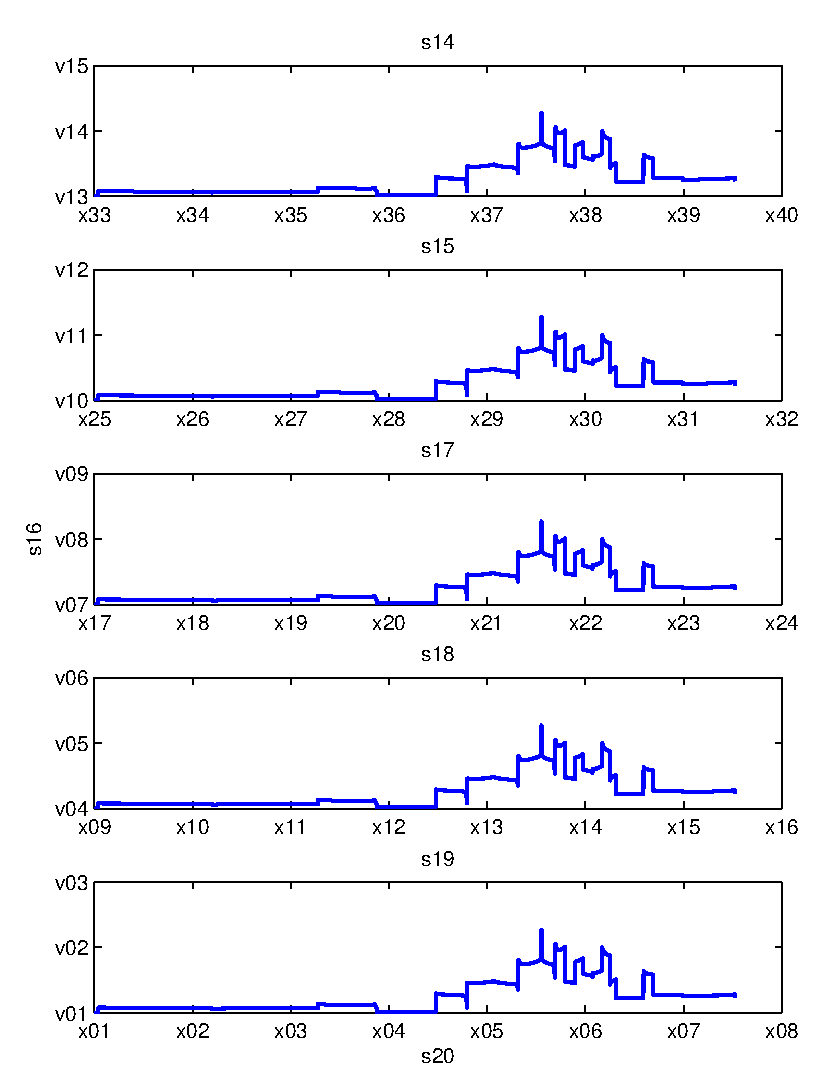
\includegraphics[width=15cm]{rmse_30_64.eps}%
\end{psfrags}%
%
% End rmse_30_64.tex
\end{document}
% See http://www.mathworks.de/matlabcentral/fileexchange/loadFile.do?objectId=4638
% for recent versions of laprint.m.
%
% created by:           LaPrint version 3.16 (13.9.2004)
% created on:           22-Apr-2014 13:13:51
% eps bounding box:     15 cm x 19.9821 cm
% comment:              
%
\begin{psfrags}%
\psfragscanon%
%
% text strings:
\psfrag{s14}[b][b]{\color[rgb]{0,0,0}\setlength{\tabcolsep}{0pt}\begin{tabular}{c}EKF\end{tabular}}%
\psfrag{s15}[b][b]{\color[rgb]{0,0,0}\setlength{\tabcolsep}{0pt}\begin{tabular}{c}UKF\end{tabular}}%
\psfrag{s16}[b][b]{\color[rgb]{0,0,0}\setlength{\tabcolsep}{0pt}\begin{tabular}{c}RMSE\end{tabular}}%
\psfrag{s17}[b][b]{\color[rgb]{0,0,0}\setlength{\tabcolsep}{0pt}\begin{tabular}{c}CKF3\end{tabular}}%
\psfrag{s18}[b][b]{\color[rgb]{0,0,0}\setlength{\tabcolsep}{0pt}\begin{tabular}{c}CKF5\end{tabular}}%
\psfrag{s19}[b][b]{\color[rgb]{0,0,0}\setlength{\tabcolsep}{0pt}\begin{tabular}{c}SLF\end{tabular}}%
\psfrag{s20}[t][t]{\color[rgb]{0,0,0}\setlength{\tabcolsep}{0pt}\begin{tabular}{c}$k$\end{tabular}}%
%
% xticklabels:
\psfrag{x01}[t][t]{0}%
\psfrag{x02}[t][t]{500}%
\psfrag{x03}[t][t]{1000}%
\psfrag{x04}[t][t]{1500}%
\psfrag{x05}[t][t]{2000}%
\psfrag{x06}[t][t]{2500}%
\psfrag{x07}[t][t]{3000}%
\psfrag{x08}[t][t]{3500}%
\psfrag{x09}[t][t]{0}%
\psfrag{x10}[t][t]{500}%
\psfrag{x11}[t][t]{1000}%
\psfrag{x12}[t][t]{1500}%
\psfrag{x13}[t][t]{2000}%
\psfrag{x14}[t][t]{2500}%
\psfrag{x15}[t][t]{3000}%
\psfrag{x16}[t][t]{3500}%
\psfrag{x17}[t][t]{0}%
\psfrag{x18}[t][t]{500}%
\psfrag{x19}[t][t]{1000}%
\psfrag{x20}[t][t]{1500}%
\psfrag{x21}[t][t]{2000}%
\psfrag{x22}[t][t]{2500}%
\psfrag{x23}[t][t]{3000}%
\psfrag{x24}[t][t]{3500}%
\psfrag{x25}[t][t]{0}%
\psfrag{x26}[t][t]{500}%
\psfrag{x27}[t][t]{1000}%
\psfrag{x28}[t][t]{1500}%
\psfrag{x29}[t][t]{2000}%
\psfrag{x30}[t][t]{2500}%
\psfrag{x31}[t][t]{3000}%
\psfrag{x32}[t][t]{3500}%
\psfrag{x33}[t][t]{0}%
\psfrag{x34}[t][t]{500}%
\psfrag{x35}[t][t]{1000}%
\psfrag{x36}[t][t]{1500}%
\psfrag{x37}[t][t]{2000}%
\psfrag{x38}[t][t]{2500}%
\psfrag{x39}[t][t]{3000}%
\psfrag{x40}[t][t]{3500}%
%
% yticklabels:
\psfrag{v01}[r][r]{0}%
\psfrag{v02}[r][r]{0.02}%
\psfrag{v03}[r][r]{0.04}%
\psfrag{v04}[r][r]{0}%
\psfrag{v05}[r][r]{0.02}%
\psfrag{v06}[r][r]{0.04}%
\psfrag{v07}[r][r]{0}%
\psfrag{v08}[r][r]{0.02}%
\psfrag{v09}[r][r]{0.04}%
\psfrag{v10}[r][r]{0}%
\psfrag{v11}[r][r]{0.02}%
\psfrag{v12}[r][r]{0.04}%
\psfrag{v13}[r][r]{0}%
\psfrag{v14}[r][r]{0.02}%
\psfrag{v15}[r][r]{0.04}%
%
% Figure:
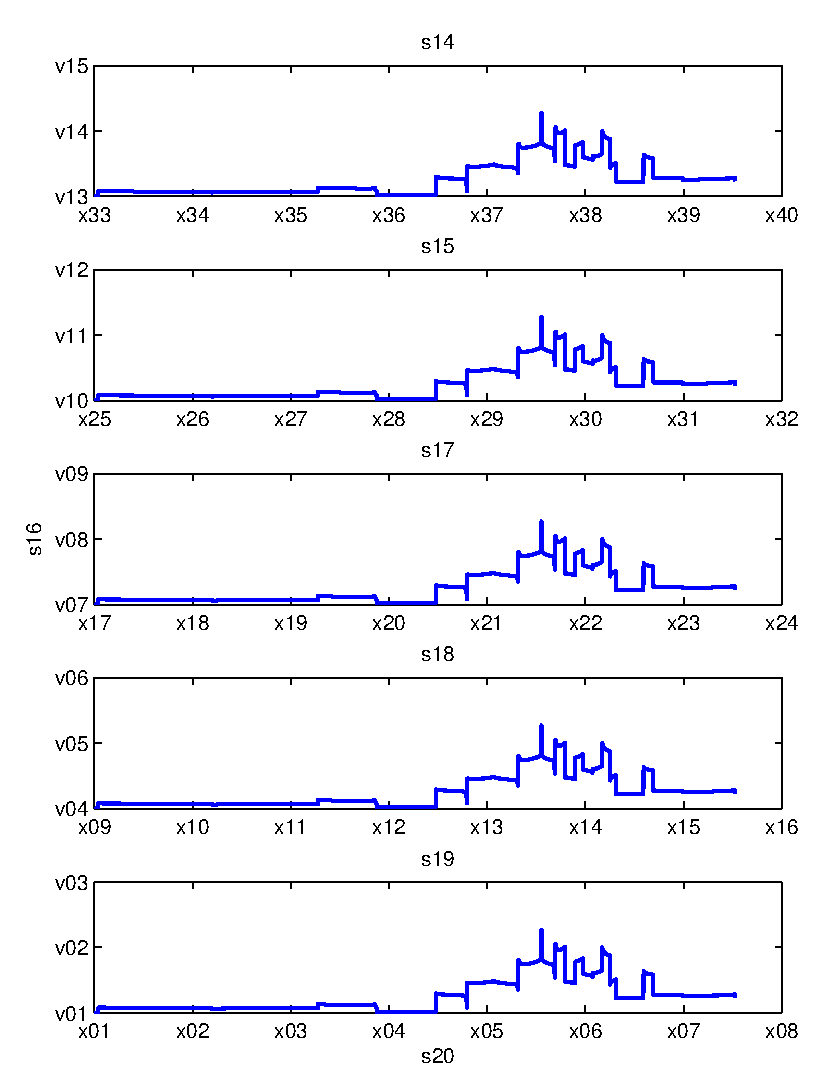
\includegraphics[width=15cm]{rmse_30_64.eps}%
\end{psfrags}%
%
% End rmse_30_64.tex

\caption{RMSE of SOC estimation for $T_s=30$~s and $M=64$.}
\label{fig:rmse_30_64}
\end{figure}

\clearpage

\section{Sampling Period of 150 Seconds}

From \cref{tab:div_150}, it can be seen that the filters have no divergences for $M=16,\dots,256$. For small $M$, all filters diverge, as expected. For large $M$, there are no divergences, unlike with $T_s=30$ seconds. The times shown in \cref{tab:time_150} show that the EKF is again the fastest with a similar ratio between the speeds as with $T_s=30$ seconds. 

\begin{table}[h]
\centering
\caption{Number of divergences in 100 Monte Carlo runs for $T_s=150$~s as a function of number of integration steps $M$}
\begin{tabular}{@{}l*{9}{c}@{}}
\toprule
Filter/$M$ & 1   & 2   & 4   & 8   & 16 & 32 & 64 & 128 & 256 \\
\midrule
EKF        & 100 & 100 & 98  & 77  & 0  & 0  & 0  & 0   & 0   \\
UKF        & 100 & 100 & 100 & 100 & 0  & 0  & 0  & 0   & 0   \\
CKF3       & 100 & 100 & 100 & 100 & 0  & 0  & 0  & 0   & 0   \\
CKF5       & 100 & 100 & 100 & 100 & 0  & 0  & 0  & 0   & 0   \\
SLF        & 100 & 100 & 100 & 100 & 0  & 0  & 0  & 0   & 0   \\
\bottomrule
\end{tabular}
\label{tab:div_150}
\end{table}

\begin{table}[h]
\centering
\caption{Filtering time in seconds for 100 Monte Carlo runs for $T_s=150$~s as a function of number of integration steps $M$}
\begin{tabular}{@{}lccccccccc@{}}
\toprule
Filter/$M$ & 1      & 2     & 4     & 8     & 16    & 32    & 64    & 128   & 256   \\ \midrule
EKF        & 0.544  & 2.359 & 6.297 & 7.787 & 3.868 & 7.753 & 15.49 & 30.97 & 61.67 \\
UKF        & 0.6749 & 1.185 & 2.414 & 6.983 & 18.81 & 37.53 & 74.89 & 149.8 & 299.2 \\
CKF        & 0.499  & 1.173 & 2.147 & 6.098 & 16.49 & 33.09 & 66.08 & 131.9 & 264.1 \\
CKF5       & 2.949  & 5.709 & 10.93 & 22.49 & 47.34 & 94.14 & 188.2 & 377.6 & 753.7 \\
SLF        & 0.873  & 1.655 & 3.217 & 6.352 & 12.7  & 25.39 & 50.63 & 101   & 201.9 \\ \bottomrule
\end{tabular}
\label{tab:time_150}
\end{table}

\cref{fig:mrmse_150} shows the MRMSE as a function of the number of integration steps over the divergence-free range. It can be seen that the errors decrease as the number of integration steps increase, and the rate of decrease is roughly the same for all five filters. The EKF results in the least error by far, with its MRMSE at $M=16$ approximately equal to the MRMSEs of the other filters at $M=256$. For small $M$, the UKF has the second smallest error with the two CKFs and the SLF having approximately the same error. For large $M$, the CKF5 and the SLF have the second smallest error, being trailed by the CKF3 and, then the UKF. For comparison purposes, the RMSE at $M=16$ and 256 are shown in \cref{fig:rmse_150_16,fig:rmse_150_256}. The RMSEs for the filters are all very close in value. It can be seen that the RMSEs increase during the period of high-rate charge and discharge, when the nonlinear effects are the strongest. These increases are less pronounced for $M=256$ than for $M=16$, as expected. The fluctuations in the RMSE occur when transitioning between charging and discharging.

\begin{figure}[b]
\centering
% This file is generated by the MATLAB m-file laprint.m. It can be included
% into LaTeX documents using the packages graphicx, color and psfrag.
% It is accompanied by a postscript file. A sample LaTeX file is:
%    \documentclass{article}\usepackage{graphicx,color,psfrag}
%    \begin{document}% This file is generated by the MATLAB m-file laprint.m. It can be included
% into LaTeX documents using the packages graphicx, color and psfrag.
% It is accompanied by a postscript file. A sample LaTeX file is:
%    \documentclass{article}\usepackage{graphicx,color,psfrag}
%    \begin{document}% This file is generated by the MATLAB m-file laprint.m. It can be included
% into LaTeX documents using the packages graphicx, color and psfrag.
% It is accompanied by a postscript file. A sample LaTeX file is:
%    \documentclass{article}\usepackage{graphicx,color,psfrag}
%    \begin{document}\input{mrmse_150}\end{document}
% See http://www.mathworks.de/matlabcentral/fileexchange/loadFile.do?objectId=4638
% for recent versions of laprint.m.
%
% created by:           LaPrint version 3.16 (13.9.2004)
% created on:           08-Apr-2014 21:55:04
% eps bounding box:     15 cm x 11.25 cm
% comment:              
%
\begin{psfrags}%
\psfragscanon%
%
% text strings:
\psfrag{s09}[t][t]{\color[rgb]{0,0,0}\setlength{\tabcolsep}{0pt}\begin{tabular}{c}$\log_2 (M) + 1$\end{tabular}}%
\psfrag{s10}[b][b]{\color[rgb]{0,0,0}\setlength{\tabcolsep}{0pt}\begin{tabular}{c}MRMSE\end{tabular}}%
\psfrag{s14}[][]{\color[rgb]{0,0,0}\setlength{\tabcolsep}{0pt}\begin{tabular}{c} \end{tabular}}%
\psfrag{s15}[][]{\color[rgb]{0,0,0}\setlength{\tabcolsep}{0pt}\begin{tabular}{c} \end{tabular}}%
\psfrag{s16}[l][l]{\color[rgb]{0,0,0}SLF}%
\psfrag{s17}[l][l]{\color[rgb]{0,0,0}EKF}%
\psfrag{s18}[l][l]{\color[rgb]{0,0,0}UKF}%
\psfrag{s19}[l][l]{\color[rgb]{0,0,0}CKF}%
\psfrag{s20}[l][l]{\color[rgb]{0,0,0}SLF}%
%
% xticklabels:
\psfrag{x01}[t][t]{0}%
\psfrag{x02}[t][t]{0.1}%
\psfrag{x03}[t][t]{0.2}%
\psfrag{x04}[t][t]{0.3}%
\psfrag{x05}[t][t]{0.4}%
\psfrag{x06}[t][t]{0.5}%
\psfrag{x07}[t][t]{0.6}%
\psfrag{x08}[t][t]{0.7}%
\psfrag{x09}[t][t]{0.8}%
\psfrag{x10}[t][t]{0.9}%
\psfrag{x11}[t][t]{1}%
\psfrag{x12}[t][t]{1}%
\psfrag{x13}[t][t]{2}%
\psfrag{x14}[t][t]{3}%
\psfrag{x15}[t][t]{4}%
\psfrag{x16}[t][t]{5}%
\psfrag{x17}[t][t]{6}%
\psfrag{x18}[t][t]{7}%
\psfrag{x19}[t][t]{8}%
\psfrag{x20}[t][t]{9}%
%
% yticklabels:
\psfrag{v01}[r][r]{0}%
\psfrag{v02}[r][r]{0.1}%
\psfrag{v03}[r][r]{0.2}%
\psfrag{v04}[r][r]{0.3}%
\psfrag{v05}[r][r]{0.4}%
\psfrag{v06}[r][r]{0.5}%
\psfrag{v07}[r][r]{0.6}%
\psfrag{v08}[r][r]{0.7}%
\psfrag{v09}[r][r]{0.8}%
\psfrag{v10}[r][r]{0.9}%
\psfrag{v11}[r][r]{1}%
\psfrag{v12}[r][r]{0}%
\psfrag{v13}[r][r]{0.05}%
\psfrag{v14}[r][r]{0.1}%
\psfrag{v15}[r][r]{0.15}%
\psfrag{v16}[r][r]{0.2}%
\psfrag{v17}[r][r]{0.25}%
\psfrag{v18}[r][r]{0.3}%
\psfrag{v19}[r][r]{0.35}%
\psfrag{v20}[r][r]{0.4}%
\psfrag{v21}[r][r]{0.45}%
\psfrag{v22}[r][r]{0.5}%
%
% Figure:
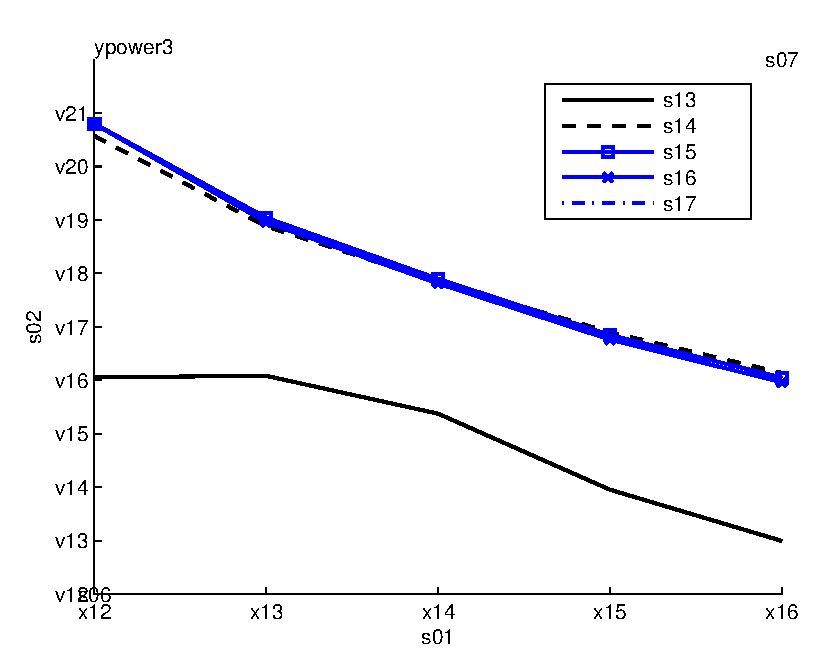
\includegraphics[width=15cm]{mrmse_150.eps}%
\end{psfrags}%
%
% End mrmse_150.tex
\end{document}
% See http://www.mathworks.de/matlabcentral/fileexchange/loadFile.do?objectId=4638
% for recent versions of laprint.m.
%
% created by:           LaPrint version 3.16 (13.9.2004)
% created on:           08-Apr-2014 21:55:04
% eps bounding box:     15 cm x 11.25 cm
% comment:              
%
\begin{psfrags}%
\psfragscanon%
%
% text strings:
\psfrag{s09}[t][t]{\color[rgb]{0,0,0}\setlength{\tabcolsep}{0pt}\begin{tabular}{c}$\log_2 (M) + 1$\end{tabular}}%
\psfrag{s10}[b][b]{\color[rgb]{0,0,0}\setlength{\tabcolsep}{0pt}\begin{tabular}{c}MRMSE\end{tabular}}%
\psfrag{s14}[][]{\color[rgb]{0,0,0}\setlength{\tabcolsep}{0pt}\begin{tabular}{c} \end{tabular}}%
\psfrag{s15}[][]{\color[rgb]{0,0,0}\setlength{\tabcolsep}{0pt}\begin{tabular}{c} \end{tabular}}%
\psfrag{s16}[l][l]{\color[rgb]{0,0,0}SLF}%
\psfrag{s17}[l][l]{\color[rgb]{0,0,0}EKF}%
\psfrag{s18}[l][l]{\color[rgb]{0,0,0}UKF}%
\psfrag{s19}[l][l]{\color[rgb]{0,0,0}CKF}%
\psfrag{s20}[l][l]{\color[rgb]{0,0,0}SLF}%
%
% xticklabels:
\psfrag{x01}[t][t]{0}%
\psfrag{x02}[t][t]{0.1}%
\psfrag{x03}[t][t]{0.2}%
\psfrag{x04}[t][t]{0.3}%
\psfrag{x05}[t][t]{0.4}%
\psfrag{x06}[t][t]{0.5}%
\psfrag{x07}[t][t]{0.6}%
\psfrag{x08}[t][t]{0.7}%
\psfrag{x09}[t][t]{0.8}%
\psfrag{x10}[t][t]{0.9}%
\psfrag{x11}[t][t]{1}%
\psfrag{x12}[t][t]{1}%
\psfrag{x13}[t][t]{2}%
\psfrag{x14}[t][t]{3}%
\psfrag{x15}[t][t]{4}%
\psfrag{x16}[t][t]{5}%
\psfrag{x17}[t][t]{6}%
\psfrag{x18}[t][t]{7}%
\psfrag{x19}[t][t]{8}%
\psfrag{x20}[t][t]{9}%
%
% yticklabels:
\psfrag{v01}[r][r]{0}%
\psfrag{v02}[r][r]{0.1}%
\psfrag{v03}[r][r]{0.2}%
\psfrag{v04}[r][r]{0.3}%
\psfrag{v05}[r][r]{0.4}%
\psfrag{v06}[r][r]{0.5}%
\psfrag{v07}[r][r]{0.6}%
\psfrag{v08}[r][r]{0.7}%
\psfrag{v09}[r][r]{0.8}%
\psfrag{v10}[r][r]{0.9}%
\psfrag{v11}[r][r]{1}%
\psfrag{v12}[r][r]{0}%
\psfrag{v13}[r][r]{0.05}%
\psfrag{v14}[r][r]{0.1}%
\psfrag{v15}[r][r]{0.15}%
\psfrag{v16}[r][r]{0.2}%
\psfrag{v17}[r][r]{0.25}%
\psfrag{v18}[r][r]{0.3}%
\psfrag{v19}[r][r]{0.35}%
\psfrag{v20}[r][r]{0.4}%
\psfrag{v21}[r][r]{0.45}%
\psfrag{v22}[r][r]{0.5}%
%
% Figure:
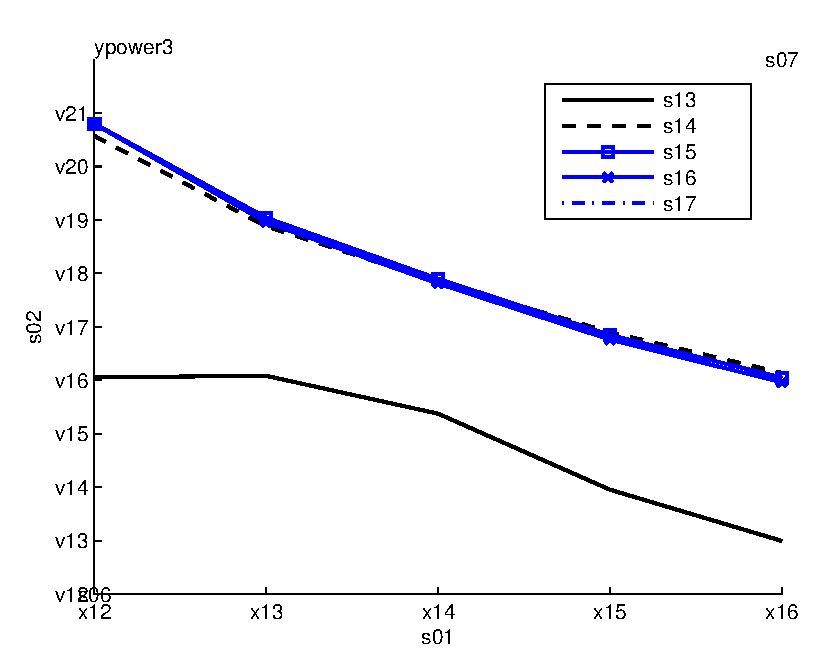
\includegraphics[width=15cm]{mrmse_150.eps}%
\end{psfrags}%
%
% End mrmse_150.tex
\end{document}
% See http://www.mathworks.de/matlabcentral/fileexchange/loadFile.do?objectId=4638
% for recent versions of laprint.m.
%
% created by:           LaPrint version 3.16 (13.9.2004)
% created on:           08-Apr-2014 21:55:04
% eps bounding box:     15 cm x 11.25 cm
% comment:              
%
\begin{psfrags}%
\psfragscanon%
%
% text strings:
\psfrag{s09}[t][t]{\color[rgb]{0,0,0}\setlength{\tabcolsep}{0pt}\begin{tabular}{c}$\log_2 (M) + 1$\end{tabular}}%
\psfrag{s10}[b][b]{\color[rgb]{0,0,0}\setlength{\tabcolsep}{0pt}\begin{tabular}{c}MRMSE\end{tabular}}%
\psfrag{s14}[][]{\color[rgb]{0,0,0}\setlength{\tabcolsep}{0pt}\begin{tabular}{c} \end{tabular}}%
\psfrag{s15}[][]{\color[rgb]{0,0,0}\setlength{\tabcolsep}{0pt}\begin{tabular}{c} \end{tabular}}%
\psfrag{s16}[l][l]{\color[rgb]{0,0,0}SLF}%
\psfrag{s17}[l][l]{\color[rgb]{0,0,0}EKF}%
\psfrag{s18}[l][l]{\color[rgb]{0,0,0}UKF}%
\psfrag{s19}[l][l]{\color[rgb]{0,0,0}CKF}%
\psfrag{s20}[l][l]{\color[rgb]{0,0,0}SLF}%
%
% xticklabels:
\psfrag{x01}[t][t]{0}%
\psfrag{x02}[t][t]{0.1}%
\psfrag{x03}[t][t]{0.2}%
\psfrag{x04}[t][t]{0.3}%
\psfrag{x05}[t][t]{0.4}%
\psfrag{x06}[t][t]{0.5}%
\psfrag{x07}[t][t]{0.6}%
\psfrag{x08}[t][t]{0.7}%
\psfrag{x09}[t][t]{0.8}%
\psfrag{x10}[t][t]{0.9}%
\psfrag{x11}[t][t]{1}%
\psfrag{x12}[t][t]{1}%
\psfrag{x13}[t][t]{2}%
\psfrag{x14}[t][t]{3}%
\psfrag{x15}[t][t]{4}%
\psfrag{x16}[t][t]{5}%
\psfrag{x17}[t][t]{6}%
\psfrag{x18}[t][t]{7}%
\psfrag{x19}[t][t]{8}%
\psfrag{x20}[t][t]{9}%
%
% yticklabels:
\psfrag{v01}[r][r]{0}%
\psfrag{v02}[r][r]{0.1}%
\psfrag{v03}[r][r]{0.2}%
\psfrag{v04}[r][r]{0.3}%
\psfrag{v05}[r][r]{0.4}%
\psfrag{v06}[r][r]{0.5}%
\psfrag{v07}[r][r]{0.6}%
\psfrag{v08}[r][r]{0.7}%
\psfrag{v09}[r][r]{0.8}%
\psfrag{v10}[r][r]{0.9}%
\psfrag{v11}[r][r]{1}%
\psfrag{v12}[r][r]{0}%
\psfrag{v13}[r][r]{0.05}%
\psfrag{v14}[r][r]{0.1}%
\psfrag{v15}[r][r]{0.15}%
\psfrag{v16}[r][r]{0.2}%
\psfrag{v17}[r][r]{0.25}%
\psfrag{v18}[r][r]{0.3}%
\psfrag{v19}[r][r]{0.35}%
\psfrag{v20}[r][r]{0.4}%
\psfrag{v21}[r][r]{0.45}%
\psfrag{v22}[r][r]{0.5}%
%
% Figure:
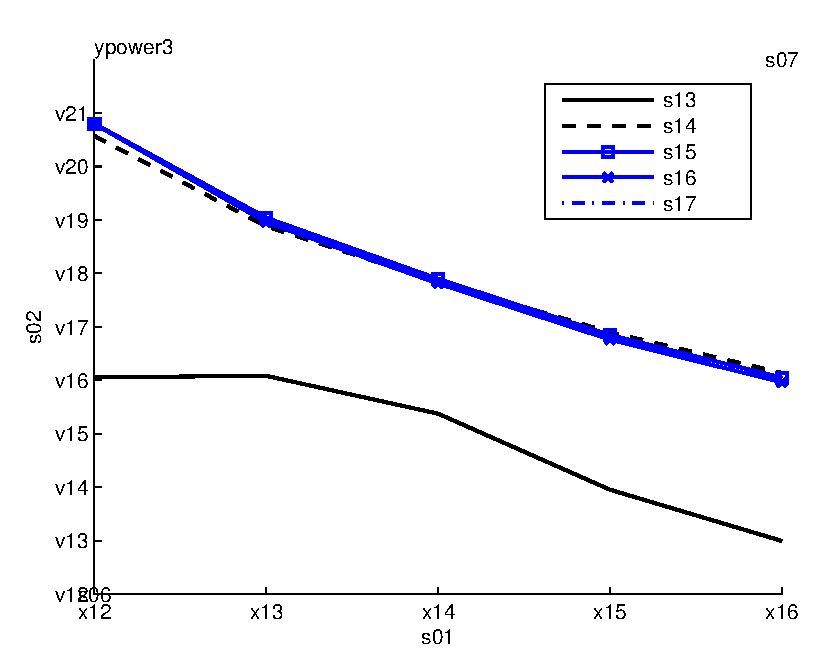
\includegraphics[width=15cm]{mrmse_150.eps}%
\end{psfrags}%
%
% End mrmse_150.tex

\caption{SOC error for $T_s=150$~s as a function of number of integration steps $M$.}
\label{fig:mrmse_150}
\end{figure}

\begin{figure}
\centering
% This file is generated by the MATLAB m-file laprint.m. It can be included
% into LaTeX documents using the packages graphicx, color and psfrag.
% It is accompanied by a postscript file. A sample LaTeX file is:
%    \documentclass{article}\usepackage{graphicx,color,psfrag}
%    \begin{document}% This file is generated by the MATLAB m-file laprint.m. It can be included
% into LaTeX documents using the packages graphicx, color and psfrag.
% It is accompanied by a postscript file. A sample LaTeX file is:
%    \documentclass{article}\usepackage{graphicx,color,psfrag}
%    \begin{document}% This file is generated by the MATLAB m-file laprint.m. It can be included
% into LaTeX documents using the packages graphicx, color and psfrag.
% It is accompanied by a postscript file. A sample LaTeX file is:
%    \documentclass{article}\usepackage{graphicx,color,psfrag}
%    \begin{document}\input{rmse_150_16}\end{document}
% See http://www.mathworks.de/matlabcentral/fileexchange/loadFile.do?objectId=4638
% for recent versions of laprint.m.
%
% created by:           LaPrint version 3.16 (13.9.2004)
% created on:           22-Apr-2014 13:35:27
% eps bounding box:     15 cm x 19.9821 cm
% comment:              
%
\begin{psfrags}%
\psfragscanon%
%
% text strings:
\psfrag{s14}[b][b]{\color[rgb]{0,0,0}\setlength{\tabcolsep}{0pt}\begin{tabular}{c}EKF\end{tabular}}%
\psfrag{s15}[b][b]{\color[rgb]{0,0,0}\setlength{\tabcolsep}{0pt}\begin{tabular}{c}UKF\end{tabular}}%
\psfrag{s16}[b][b]{\color[rgb]{0,0,0}\setlength{\tabcolsep}{0pt}\begin{tabular}{c}RMSE\end{tabular}}%
\psfrag{s17}[b][b]{\color[rgb]{0,0,0}\setlength{\tabcolsep}{0pt}\begin{tabular}{c}CKF3\end{tabular}}%
\psfrag{s18}[b][b]{\color[rgb]{0,0,0}\setlength{\tabcolsep}{0pt}\begin{tabular}{c}CKF5\end{tabular}}%
\psfrag{s19}[b][b]{\color[rgb]{0,0,0}\setlength{\tabcolsep}{0pt}\begin{tabular}{c}SLF\end{tabular}}%
\psfrag{s20}[t][t]{\color[rgb]{0,0,0}\setlength{\tabcolsep}{0pt}\begin{tabular}{c}$k$\end{tabular}}%
%
% xticklabels:
\psfrag{x01}[t][t]{0}%
\psfrag{x02}[t][t]{100}%
\psfrag{x03}[t][t]{200}%
\psfrag{x04}[t][t]{300}%
\psfrag{x05}[t][t]{400}%
\psfrag{x06}[t][t]{500}%
\psfrag{x07}[t][t]{600}%
\psfrag{x08}[t][t]{700}%
\psfrag{x09}[t][t]{0}%
\psfrag{x10}[t][t]{100}%
\psfrag{x11}[t][t]{200}%
\psfrag{x12}[t][t]{300}%
\psfrag{x13}[t][t]{400}%
\psfrag{x14}[t][t]{500}%
\psfrag{x15}[t][t]{600}%
\psfrag{x16}[t][t]{700}%
\psfrag{x17}[t][t]{0}%
\psfrag{x18}[t][t]{100}%
\psfrag{x19}[t][t]{200}%
\psfrag{x20}[t][t]{300}%
\psfrag{x21}[t][t]{400}%
\psfrag{x22}[t][t]{500}%
\psfrag{x23}[t][t]{600}%
\psfrag{x24}[t][t]{700}%
\psfrag{x25}[t][t]{0}%
\psfrag{x26}[t][t]{100}%
\psfrag{x27}[t][t]{200}%
\psfrag{x28}[t][t]{300}%
\psfrag{x29}[t][t]{400}%
\psfrag{x30}[t][t]{500}%
\psfrag{x31}[t][t]{600}%
\psfrag{x32}[t][t]{700}%
\psfrag{x33}[t][t]{0}%
\psfrag{x34}[t][t]{100}%
\psfrag{x35}[t][t]{200}%
\psfrag{x36}[t][t]{300}%
\psfrag{x37}[t][t]{400}%
\psfrag{x38}[t][t]{500}%
\psfrag{x39}[t][t]{600}%
\psfrag{x40}[t][t]{700}%
%
% yticklabels:
\psfrag{v01}[r][r]{0}%
\psfrag{v02}[r][r]{0.02}%
\psfrag{v03}[r][r]{0.04}%
\psfrag{v04}[r][r]{0}%
\psfrag{v05}[r][r]{0.02}%
\psfrag{v06}[r][r]{0.04}%
\psfrag{v07}[r][r]{0}%
\psfrag{v08}[r][r]{0.02}%
\psfrag{v09}[r][r]{0.04}%
\psfrag{v10}[r][r]{0}%
\psfrag{v11}[r][r]{0.02}%
\psfrag{v12}[r][r]{0.04}%
\psfrag{v13}[r][r]{0}%
\psfrag{v14}[r][r]{0.02}%
\psfrag{v15}[r][r]{0.04}%
%
% Figure:
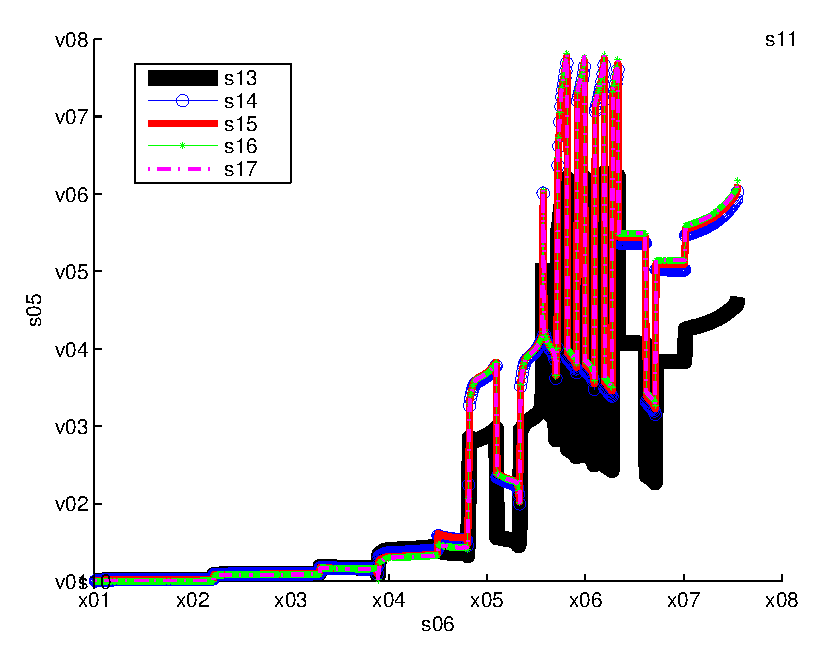
\includegraphics[width=15cm]{rmse_150_16.eps}%
\end{psfrags}%
%
% End rmse_150_16.tex
\end{document}
% See http://www.mathworks.de/matlabcentral/fileexchange/loadFile.do?objectId=4638
% for recent versions of laprint.m.
%
% created by:           LaPrint version 3.16 (13.9.2004)
% created on:           22-Apr-2014 13:35:27
% eps bounding box:     15 cm x 19.9821 cm
% comment:              
%
\begin{psfrags}%
\psfragscanon%
%
% text strings:
\psfrag{s14}[b][b]{\color[rgb]{0,0,0}\setlength{\tabcolsep}{0pt}\begin{tabular}{c}EKF\end{tabular}}%
\psfrag{s15}[b][b]{\color[rgb]{0,0,0}\setlength{\tabcolsep}{0pt}\begin{tabular}{c}UKF\end{tabular}}%
\psfrag{s16}[b][b]{\color[rgb]{0,0,0}\setlength{\tabcolsep}{0pt}\begin{tabular}{c}RMSE\end{tabular}}%
\psfrag{s17}[b][b]{\color[rgb]{0,0,0}\setlength{\tabcolsep}{0pt}\begin{tabular}{c}CKF3\end{tabular}}%
\psfrag{s18}[b][b]{\color[rgb]{0,0,0}\setlength{\tabcolsep}{0pt}\begin{tabular}{c}CKF5\end{tabular}}%
\psfrag{s19}[b][b]{\color[rgb]{0,0,0}\setlength{\tabcolsep}{0pt}\begin{tabular}{c}SLF\end{tabular}}%
\psfrag{s20}[t][t]{\color[rgb]{0,0,0}\setlength{\tabcolsep}{0pt}\begin{tabular}{c}$k$\end{tabular}}%
%
% xticklabels:
\psfrag{x01}[t][t]{0}%
\psfrag{x02}[t][t]{100}%
\psfrag{x03}[t][t]{200}%
\psfrag{x04}[t][t]{300}%
\psfrag{x05}[t][t]{400}%
\psfrag{x06}[t][t]{500}%
\psfrag{x07}[t][t]{600}%
\psfrag{x08}[t][t]{700}%
\psfrag{x09}[t][t]{0}%
\psfrag{x10}[t][t]{100}%
\psfrag{x11}[t][t]{200}%
\psfrag{x12}[t][t]{300}%
\psfrag{x13}[t][t]{400}%
\psfrag{x14}[t][t]{500}%
\psfrag{x15}[t][t]{600}%
\psfrag{x16}[t][t]{700}%
\psfrag{x17}[t][t]{0}%
\psfrag{x18}[t][t]{100}%
\psfrag{x19}[t][t]{200}%
\psfrag{x20}[t][t]{300}%
\psfrag{x21}[t][t]{400}%
\psfrag{x22}[t][t]{500}%
\psfrag{x23}[t][t]{600}%
\psfrag{x24}[t][t]{700}%
\psfrag{x25}[t][t]{0}%
\psfrag{x26}[t][t]{100}%
\psfrag{x27}[t][t]{200}%
\psfrag{x28}[t][t]{300}%
\psfrag{x29}[t][t]{400}%
\psfrag{x30}[t][t]{500}%
\psfrag{x31}[t][t]{600}%
\psfrag{x32}[t][t]{700}%
\psfrag{x33}[t][t]{0}%
\psfrag{x34}[t][t]{100}%
\psfrag{x35}[t][t]{200}%
\psfrag{x36}[t][t]{300}%
\psfrag{x37}[t][t]{400}%
\psfrag{x38}[t][t]{500}%
\psfrag{x39}[t][t]{600}%
\psfrag{x40}[t][t]{700}%
%
% yticklabels:
\psfrag{v01}[r][r]{0}%
\psfrag{v02}[r][r]{0.02}%
\psfrag{v03}[r][r]{0.04}%
\psfrag{v04}[r][r]{0}%
\psfrag{v05}[r][r]{0.02}%
\psfrag{v06}[r][r]{0.04}%
\psfrag{v07}[r][r]{0}%
\psfrag{v08}[r][r]{0.02}%
\psfrag{v09}[r][r]{0.04}%
\psfrag{v10}[r][r]{0}%
\psfrag{v11}[r][r]{0.02}%
\psfrag{v12}[r][r]{0.04}%
\psfrag{v13}[r][r]{0}%
\psfrag{v14}[r][r]{0.02}%
\psfrag{v15}[r][r]{0.04}%
%
% Figure:
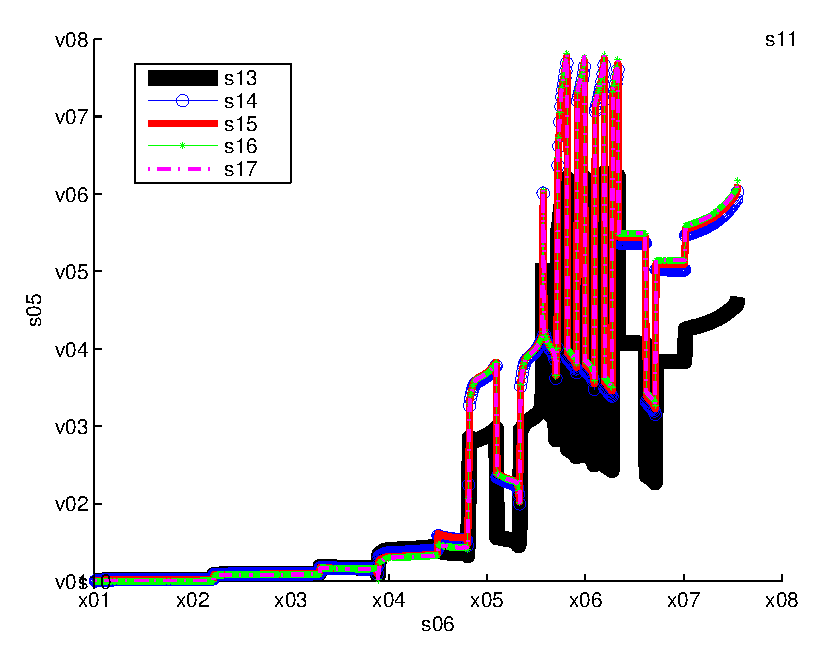
\includegraphics[width=15cm]{rmse_150_16.eps}%
\end{psfrags}%
%
% End rmse_150_16.tex
\end{document}
% See http://www.mathworks.de/matlabcentral/fileexchange/loadFile.do?objectId=4638
% for recent versions of laprint.m.
%
% created by:           LaPrint version 3.16 (13.9.2004)
% created on:           22-Apr-2014 13:35:27
% eps bounding box:     15 cm x 19.9821 cm
% comment:              
%
\begin{psfrags}%
\psfragscanon%
%
% text strings:
\psfrag{s14}[b][b]{\color[rgb]{0,0,0}\setlength{\tabcolsep}{0pt}\begin{tabular}{c}EKF\end{tabular}}%
\psfrag{s15}[b][b]{\color[rgb]{0,0,0}\setlength{\tabcolsep}{0pt}\begin{tabular}{c}UKF\end{tabular}}%
\psfrag{s16}[b][b]{\color[rgb]{0,0,0}\setlength{\tabcolsep}{0pt}\begin{tabular}{c}RMSE\end{tabular}}%
\psfrag{s17}[b][b]{\color[rgb]{0,0,0}\setlength{\tabcolsep}{0pt}\begin{tabular}{c}CKF3\end{tabular}}%
\psfrag{s18}[b][b]{\color[rgb]{0,0,0}\setlength{\tabcolsep}{0pt}\begin{tabular}{c}CKF5\end{tabular}}%
\psfrag{s19}[b][b]{\color[rgb]{0,0,0}\setlength{\tabcolsep}{0pt}\begin{tabular}{c}SLF\end{tabular}}%
\psfrag{s20}[t][t]{\color[rgb]{0,0,0}\setlength{\tabcolsep}{0pt}\begin{tabular}{c}$k$\end{tabular}}%
%
% xticklabels:
\psfrag{x01}[t][t]{0}%
\psfrag{x02}[t][t]{100}%
\psfrag{x03}[t][t]{200}%
\psfrag{x04}[t][t]{300}%
\psfrag{x05}[t][t]{400}%
\psfrag{x06}[t][t]{500}%
\psfrag{x07}[t][t]{600}%
\psfrag{x08}[t][t]{700}%
\psfrag{x09}[t][t]{0}%
\psfrag{x10}[t][t]{100}%
\psfrag{x11}[t][t]{200}%
\psfrag{x12}[t][t]{300}%
\psfrag{x13}[t][t]{400}%
\psfrag{x14}[t][t]{500}%
\psfrag{x15}[t][t]{600}%
\psfrag{x16}[t][t]{700}%
\psfrag{x17}[t][t]{0}%
\psfrag{x18}[t][t]{100}%
\psfrag{x19}[t][t]{200}%
\psfrag{x20}[t][t]{300}%
\psfrag{x21}[t][t]{400}%
\psfrag{x22}[t][t]{500}%
\psfrag{x23}[t][t]{600}%
\psfrag{x24}[t][t]{700}%
\psfrag{x25}[t][t]{0}%
\psfrag{x26}[t][t]{100}%
\psfrag{x27}[t][t]{200}%
\psfrag{x28}[t][t]{300}%
\psfrag{x29}[t][t]{400}%
\psfrag{x30}[t][t]{500}%
\psfrag{x31}[t][t]{600}%
\psfrag{x32}[t][t]{700}%
\psfrag{x33}[t][t]{0}%
\psfrag{x34}[t][t]{100}%
\psfrag{x35}[t][t]{200}%
\psfrag{x36}[t][t]{300}%
\psfrag{x37}[t][t]{400}%
\psfrag{x38}[t][t]{500}%
\psfrag{x39}[t][t]{600}%
\psfrag{x40}[t][t]{700}%
%
% yticklabels:
\psfrag{v01}[r][r]{0}%
\psfrag{v02}[r][r]{0.02}%
\psfrag{v03}[r][r]{0.04}%
\psfrag{v04}[r][r]{0}%
\psfrag{v05}[r][r]{0.02}%
\psfrag{v06}[r][r]{0.04}%
\psfrag{v07}[r][r]{0}%
\psfrag{v08}[r][r]{0.02}%
\psfrag{v09}[r][r]{0.04}%
\psfrag{v10}[r][r]{0}%
\psfrag{v11}[r][r]{0.02}%
\psfrag{v12}[r][r]{0.04}%
\psfrag{v13}[r][r]{0}%
\psfrag{v14}[r][r]{0.02}%
\psfrag{v15}[r][r]{0.04}%
%
% Figure:
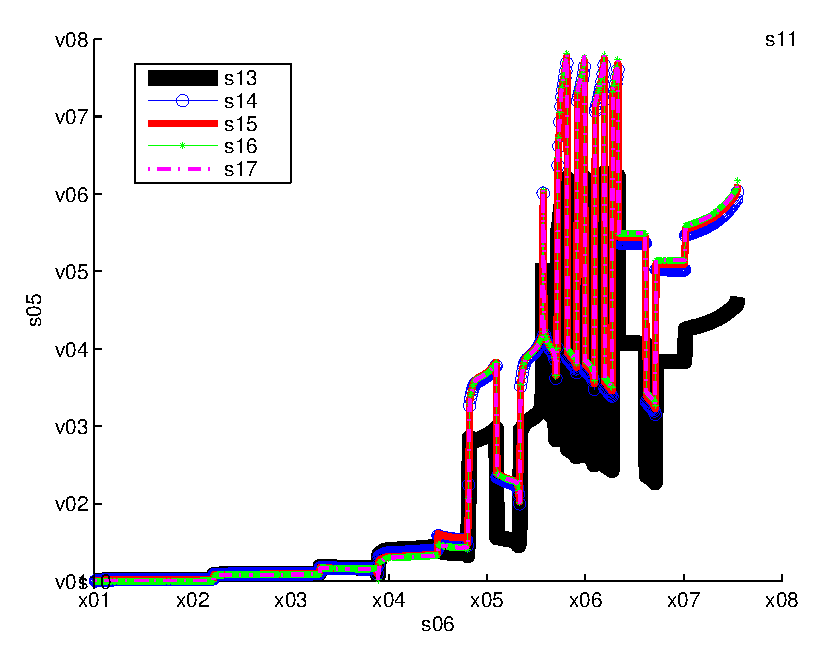
\includegraphics[width=15cm]{rmse_150_16.eps}%
\end{psfrags}%
%
% End rmse_150_16.tex

\caption{RMSE of SOC estimation for $T_s=150$~s and $M=16$.}
\label{fig:rmse_150_16}
\end{figure}

\begin{figure}
\centering
% generated by laprint.m
%
%
% text strings:
\psfrag{s05}[b][b]{\color[rgb]{0,0,0}\setlength{\tabcolsep}{0pt}\begin{tabular}{c}RMSE\end{tabular}}%
\psfrag{s06}[t][t]{\color[rgb]{0,0,0}\setlength{\tabcolsep}{0pt}\begin{tabular}{c}$k$\end{tabular}}%
\psfrag{s10}[][]{\color[rgb]{0,0,0}\setlength{\tabcolsep}{0pt}\begin{tabular}{c} \end{tabular}}%
\psfrag{s11}[][]{\color[rgb]{0,0,0}\setlength{\tabcolsep}{0pt}\begin{tabular}{c} \end{tabular}}%
\psfrag{s12}[l][l]{\color[rgb]{0,0,0}SLF}%
\psfrag{s13}[l][l]{\color[rgb]{0,0,0}EKF}%
\psfrag{s14}[l][l]{\color[rgb]{0,0,0}UKF}%
\psfrag{s15}[l][l]{\color[rgb]{0,0,0}CKF3}%
\psfrag{s16}[l][l]{\color[rgb]{0,0,0}CKF5}%
\psfrag{s17}[l][l]{\color[rgb]{0,0,0}SLF}%
%
% xticklabels:
\psfrag{x01}[t][t]{0}%
\psfrag{x02}[t][t]{100}%
\psfrag{x03}[t][t]{200}%
\psfrag{x04}[t][t]{300}%
\psfrag{x05}[t][t]{400}%
\psfrag{x06}[t][t]{500}%
\psfrag{x07}[t][t]{600}%
\psfrag{x08}[t][t]{700}%
%
% yticklabels:
\psfrag{v01}[r][r]{0}%
\psfrag{v02}[r][r]{0.005}%
\psfrag{v03}[r][r]{0.01}%
\psfrag{v04}[r][r]{0.015}%
\psfrag{v05}[r][r]{0.02}%
\psfrag{v06}[r][r]{0.025}%
\psfrag{v07}[r][r]{0.03}%
%
% Figure:
%
% End rmse_150_256.tex

\caption{RMSE of SOC estimation for $T_s=150$~s and $M=256$.}
\label{fig:rmse_150_256}
\end{figure}

\clearpage

\section{Sampling Period of 300 Seconds}

From \cref{tab:div_300}, it can be seen that the filters have no divergences for $M=64,\dots,256$. It can be seen that the UKF has more numerical problems for small $M$than the CKF3. The CKF5 and SLF are the best in terms of divergences. The times shown in \cref{tab:time_300} show that the EKF is again the fastest with a similar ratio between the speeds as with $T_s=30$ seconds. 

\begin{table}[h]
\centering
\caption{Number of divergences in 100 Monte Carlo runs for $T_s=300$~s as a function of number of integration steps $M$}
\begin{tabular}{@{}l*{9}{c}@{}}
\toprule
Filter/$M$ & 1   & 2   & 4   & 8   & 16  & 32 & 64 & 128 & 256 \\
\midrule
EKF        & 100 & 100 & 100 & 100 & 71  & 0  & 0  & 0   & 0   \\
UKF        & 100 & 100 & 100 & 100 & 99  & 5  & 0  & 0   & 0   \\
CKF3       & 100 & 100 & 100 & 100 & 99  & 0  & 0  & 0   & 0   \\
CKF5       & 100 & 100 & 100 & 100 & 0   & 0  & 0  & 0   & 0   \\
SLF        & 100 & 100 & 100 & 100 & 0   & 0  & 0  & 0   & 0   \\
\bottomrule
\end{tabular}
\label{tab:div_300}
\end{table}

\begin{table}[h]
\centering
\caption{Filtering time in seconds for 100 Monte Carlo runs for $T_s=300$~s as a function of number of integration steps $M$}
\begin{tabular}{@{}lccccccccc@{}}
\toprule
Filter/$M$ & 1     & 2     & 4     & 8     & 16    & 32    & 64    & 128   & 256   \\ \midrule
EKF        & 0.39  & 0.763 & 2.998 & 7.169 & 8.21  & 3.969 & 7.582 & 15.22 & 30.4  \\
UKF        & 0.39  & 0.578 & 1.151 & 2.276 & 6.925 & 18.55 & 37.52 & 75.1  & 150.1 \\
CKF        & 0.328 & 0.45  & 0.872 & 1.807 & 6.175 & 16.52 & 33.16 & 66.35 & 132.1 \\
CKF5       & 1.532 & 2.908 & 5.31  & 11.12 & 23.65 & 47.23 & 94.11 & 188.1 & 376.5 \\
SLF        & 0.498 & 0.958 & 1.564 & 3.114 & 6.309 & 12.71 & 25.3  & 50.47 & 101.1 \\ \bottomrule
\end{tabular}
\label{tab:time_300}
\end{table}

\cref{fig:mrmse_300} shows the MRMSE as a function of the number of integration steps over the divergence-free range. It can be seen that the errors decrease as the number of integration steps increase, and the rate of decrease is roughly the same for four of the filters, while the decrease shown by the EKF is less steep. The EKF results in the least error by far, with its MRMSE lower than those of the other filters for all combinations of $M$ in the divergence-free range. For small $M$, the UKF has the second smallest error, followed by the CKF5 and the SLF, and then the CKF3. For large $M$, the CKF5 and the SLF have the second smallest error, being trailed by the CKF3 and, then the UKF. For comparison purposes, the RMSE at $M=64$ and 256 are shown in \cref{fig:rmse_300_64,fig:rmse_300_256}. As with the other two sampling periods, the RMSEs are all very close in value. Again, the RMSEs increase during the period of high-rate charge and discharge, when the nonlinear effects are the strongest, and these increases are less pronounced for $M=256$ than for $M=16$, as expected.

\begin{figure}[b]
\centering
% This file is generated by the MATLAB m-file laprint.m. It can be included
% into LaTeX documents using the packages graphicx, color and psfrag.
% It is accompanied by a postscript file. A sample LaTeX file is:
%    \documentclass{article}\usepackage{graphicx,color,psfrag}
%    \begin{document}% This file is generated by the MATLAB m-file laprint.m. It can be included
% into LaTeX documents using the packages graphicx, color and psfrag.
% It is accompanied by a postscript file. A sample LaTeX file is:
%    \documentclass{article}\usepackage{graphicx,color,psfrag}
%    \begin{document}% This file is generated by the MATLAB m-file laprint.m. It can be included
% into LaTeX documents using the packages graphicx, color and psfrag.
% It is accompanied by a postscript file. A sample LaTeX file is:
%    \documentclass{article}\usepackage{graphicx,color,psfrag}
%    \begin{document}\input{mrmse_300}\end{document}
% See http://www.mathworks.de/matlabcentral/fileexchange/loadFile.do?objectId=4638
% for recent versions of laprint.m.
%
% created by:           LaPrint version 3.16 (13.9.2004)
% created on:           08-Apr-2014 21:59:07
% eps bounding box:     15 cm x 11.25 cm
% comment:              
%
\begin{psfrags}%
\psfragscanon%
%
% text strings:
\psfrag{s09}[t][t]{\color[rgb]{0,0,0}\setlength{\tabcolsep}{0pt}\begin{tabular}{c}$\log_2 (M) + 1$\end{tabular}}%
\psfrag{s10}[b][b]{\color[rgb]{0,0,0}\setlength{\tabcolsep}{0pt}\begin{tabular}{c}MRMSE\end{tabular}}%
\psfrag{s14}[][]{\color[rgb]{0,0,0}\setlength{\tabcolsep}{0pt}\begin{tabular}{c} \end{tabular}}%
\psfrag{s15}[][]{\color[rgb]{0,0,0}\setlength{\tabcolsep}{0pt}\begin{tabular}{c} \end{tabular}}%
\psfrag{s16}[l][l]{\color[rgb]{0,0,0}SLF}%
\psfrag{s17}[l][l]{\color[rgb]{0,0,0}EKF}%
\psfrag{s18}[l][l]{\color[rgb]{0,0,0}UKF}%
\psfrag{s19}[l][l]{\color[rgb]{0,0,0}CKF}%
\psfrag{s20}[l][l]{\color[rgb]{0,0,0}SLF}%
%
% xticklabels:
\psfrag{x01}[t][t]{0}%
\psfrag{x02}[t][t]{0.1}%
\psfrag{x03}[t][t]{0.2}%
\psfrag{x04}[t][t]{0.3}%
\psfrag{x05}[t][t]{0.4}%
\psfrag{x06}[t][t]{0.5}%
\psfrag{x07}[t][t]{0.6}%
\psfrag{x08}[t][t]{0.7}%
\psfrag{x09}[t][t]{0.8}%
\psfrag{x10}[t][t]{0.9}%
\psfrag{x11}[t][t]{1}%
\psfrag{x12}[t][t]{1}%
\psfrag{x13}[t][t]{2}%
\psfrag{x14}[t][t]{3}%
\psfrag{x15}[t][t]{4}%
\psfrag{x16}[t][t]{5}%
\psfrag{x17}[t][t]{6}%
\psfrag{x18}[t][t]{7}%
\psfrag{x19}[t][t]{8}%
\psfrag{x20}[t][t]{9}%
%
% yticklabels:
\psfrag{v01}[r][r]{0}%
\psfrag{v02}[r][r]{0.1}%
\psfrag{v03}[r][r]{0.2}%
\psfrag{v04}[r][r]{0.3}%
\psfrag{v05}[r][r]{0.4}%
\psfrag{v06}[r][r]{0.5}%
\psfrag{v07}[r][r]{0.6}%
\psfrag{v08}[r][r]{0.7}%
\psfrag{v09}[r][r]{0.8}%
\psfrag{v10}[r][r]{0.9}%
\psfrag{v11}[r][r]{1}%
\psfrag{v12}[r][r]{0}%
\psfrag{v13}[r][r]{0.05}%
\psfrag{v14}[r][r]{0.1}%
\psfrag{v15}[r][r]{0.15}%
\psfrag{v16}[r][r]{0.2}%
\psfrag{v17}[r][r]{0.25}%
\psfrag{v18}[r][r]{0.3}%
\psfrag{v19}[r][r]{0.35}%
\psfrag{v20}[r][r]{0.4}%
\psfrag{v21}[r][r]{0.45}%
\psfrag{v22}[r][r]{0.5}%
%
% Figure:
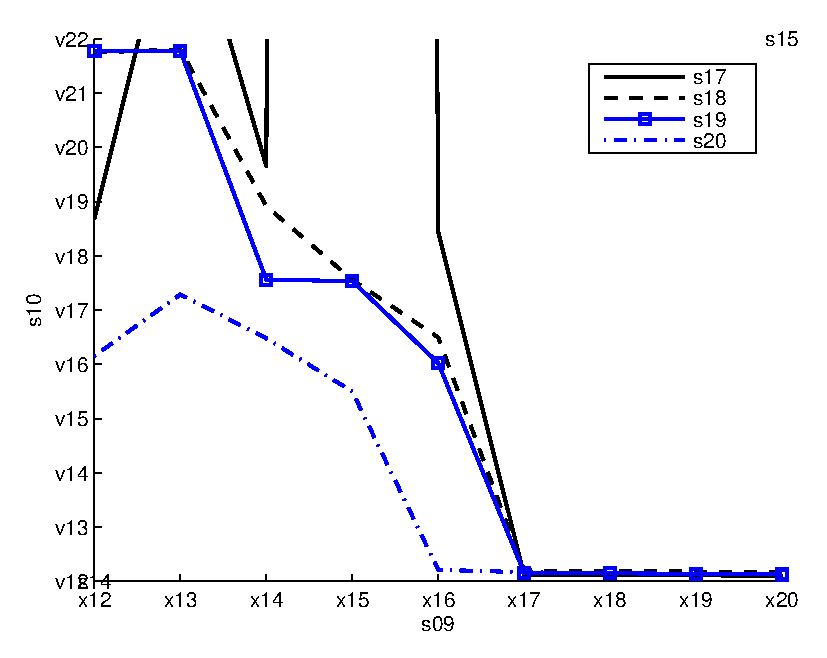
\includegraphics[width=15cm]{mrmse_300.eps}%
\end{psfrags}%
%
% End mrmse_300.tex
\end{document}
% See http://www.mathworks.de/matlabcentral/fileexchange/loadFile.do?objectId=4638
% for recent versions of laprint.m.
%
% created by:           LaPrint version 3.16 (13.9.2004)
% created on:           08-Apr-2014 21:59:07
% eps bounding box:     15 cm x 11.25 cm
% comment:              
%
\begin{psfrags}%
\psfragscanon%
%
% text strings:
\psfrag{s09}[t][t]{\color[rgb]{0,0,0}\setlength{\tabcolsep}{0pt}\begin{tabular}{c}$\log_2 (M) + 1$\end{tabular}}%
\psfrag{s10}[b][b]{\color[rgb]{0,0,0}\setlength{\tabcolsep}{0pt}\begin{tabular}{c}MRMSE\end{tabular}}%
\psfrag{s14}[][]{\color[rgb]{0,0,0}\setlength{\tabcolsep}{0pt}\begin{tabular}{c} \end{tabular}}%
\psfrag{s15}[][]{\color[rgb]{0,0,0}\setlength{\tabcolsep}{0pt}\begin{tabular}{c} \end{tabular}}%
\psfrag{s16}[l][l]{\color[rgb]{0,0,0}SLF}%
\psfrag{s17}[l][l]{\color[rgb]{0,0,0}EKF}%
\psfrag{s18}[l][l]{\color[rgb]{0,0,0}UKF}%
\psfrag{s19}[l][l]{\color[rgb]{0,0,0}CKF}%
\psfrag{s20}[l][l]{\color[rgb]{0,0,0}SLF}%
%
% xticklabels:
\psfrag{x01}[t][t]{0}%
\psfrag{x02}[t][t]{0.1}%
\psfrag{x03}[t][t]{0.2}%
\psfrag{x04}[t][t]{0.3}%
\psfrag{x05}[t][t]{0.4}%
\psfrag{x06}[t][t]{0.5}%
\psfrag{x07}[t][t]{0.6}%
\psfrag{x08}[t][t]{0.7}%
\psfrag{x09}[t][t]{0.8}%
\psfrag{x10}[t][t]{0.9}%
\psfrag{x11}[t][t]{1}%
\psfrag{x12}[t][t]{1}%
\psfrag{x13}[t][t]{2}%
\psfrag{x14}[t][t]{3}%
\psfrag{x15}[t][t]{4}%
\psfrag{x16}[t][t]{5}%
\psfrag{x17}[t][t]{6}%
\psfrag{x18}[t][t]{7}%
\psfrag{x19}[t][t]{8}%
\psfrag{x20}[t][t]{9}%
%
% yticklabels:
\psfrag{v01}[r][r]{0}%
\psfrag{v02}[r][r]{0.1}%
\psfrag{v03}[r][r]{0.2}%
\psfrag{v04}[r][r]{0.3}%
\psfrag{v05}[r][r]{0.4}%
\psfrag{v06}[r][r]{0.5}%
\psfrag{v07}[r][r]{0.6}%
\psfrag{v08}[r][r]{0.7}%
\psfrag{v09}[r][r]{0.8}%
\psfrag{v10}[r][r]{0.9}%
\psfrag{v11}[r][r]{1}%
\psfrag{v12}[r][r]{0}%
\psfrag{v13}[r][r]{0.05}%
\psfrag{v14}[r][r]{0.1}%
\psfrag{v15}[r][r]{0.15}%
\psfrag{v16}[r][r]{0.2}%
\psfrag{v17}[r][r]{0.25}%
\psfrag{v18}[r][r]{0.3}%
\psfrag{v19}[r][r]{0.35}%
\psfrag{v20}[r][r]{0.4}%
\psfrag{v21}[r][r]{0.45}%
\psfrag{v22}[r][r]{0.5}%
%
% Figure:
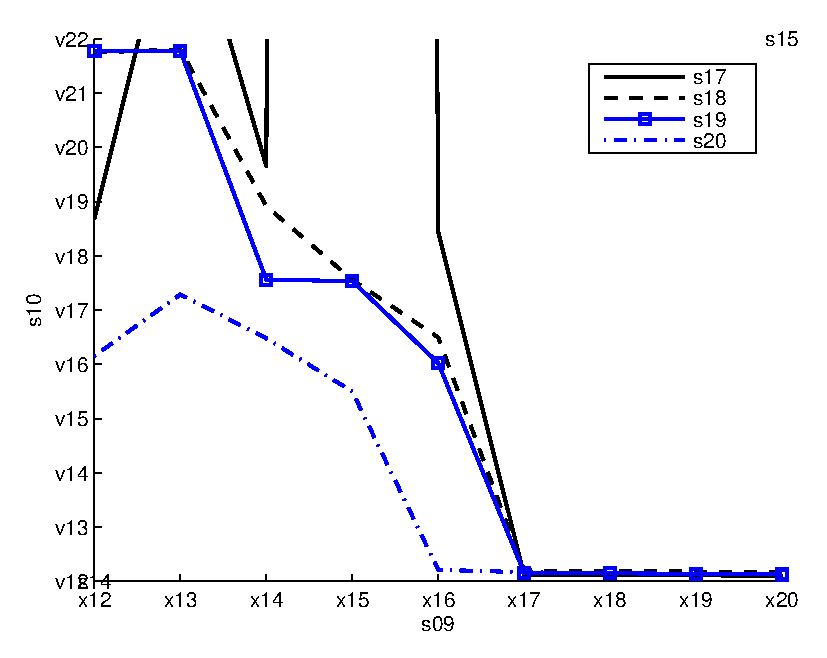
\includegraphics[width=15cm]{mrmse_300.eps}%
\end{psfrags}%
%
% End mrmse_300.tex
\end{document}
% See http://www.mathworks.de/matlabcentral/fileexchange/loadFile.do?objectId=4638
% for recent versions of laprint.m.
%
% created by:           LaPrint version 3.16 (13.9.2004)
% created on:           08-Apr-2014 21:59:07
% eps bounding box:     15 cm x 11.25 cm
% comment:              
%
\begin{psfrags}%
\psfragscanon%
%
% text strings:
\psfrag{s09}[t][t]{\color[rgb]{0,0,0}\setlength{\tabcolsep}{0pt}\begin{tabular}{c}$\log_2 (M) + 1$\end{tabular}}%
\psfrag{s10}[b][b]{\color[rgb]{0,0,0}\setlength{\tabcolsep}{0pt}\begin{tabular}{c}MRMSE\end{tabular}}%
\psfrag{s14}[][]{\color[rgb]{0,0,0}\setlength{\tabcolsep}{0pt}\begin{tabular}{c} \end{tabular}}%
\psfrag{s15}[][]{\color[rgb]{0,0,0}\setlength{\tabcolsep}{0pt}\begin{tabular}{c} \end{tabular}}%
\psfrag{s16}[l][l]{\color[rgb]{0,0,0}SLF}%
\psfrag{s17}[l][l]{\color[rgb]{0,0,0}EKF}%
\psfrag{s18}[l][l]{\color[rgb]{0,0,0}UKF}%
\psfrag{s19}[l][l]{\color[rgb]{0,0,0}CKF}%
\psfrag{s20}[l][l]{\color[rgb]{0,0,0}SLF}%
%
% xticklabels:
\psfrag{x01}[t][t]{0}%
\psfrag{x02}[t][t]{0.1}%
\psfrag{x03}[t][t]{0.2}%
\psfrag{x04}[t][t]{0.3}%
\psfrag{x05}[t][t]{0.4}%
\psfrag{x06}[t][t]{0.5}%
\psfrag{x07}[t][t]{0.6}%
\psfrag{x08}[t][t]{0.7}%
\psfrag{x09}[t][t]{0.8}%
\psfrag{x10}[t][t]{0.9}%
\psfrag{x11}[t][t]{1}%
\psfrag{x12}[t][t]{1}%
\psfrag{x13}[t][t]{2}%
\psfrag{x14}[t][t]{3}%
\psfrag{x15}[t][t]{4}%
\psfrag{x16}[t][t]{5}%
\psfrag{x17}[t][t]{6}%
\psfrag{x18}[t][t]{7}%
\psfrag{x19}[t][t]{8}%
\psfrag{x20}[t][t]{9}%
%
% yticklabels:
\psfrag{v01}[r][r]{0}%
\psfrag{v02}[r][r]{0.1}%
\psfrag{v03}[r][r]{0.2}%
\psfrag{v04}[r][r]{0.3}%
\psfrag{v05}[r][r]{0.4}%
\psfrag{v06}[r][r]{0.5}%
\psfrag{v07}[r][r]{0.6}%
\psfrag{v08}[r][r]{0.7}%
\psfrag{v09}[r][r]{0.8}%
\psfrag{v10}[r][r]{0.9}%
\psfrag{v11}[r][r]{1}%
\psfrag{v12}[r][r]{0}%
\psfrag{v13}[r][r]{0.05}%
\psfrag{v14}[r][r]{0.1}%
\psfrag{v15}[r][r]{0.15}%
\psfrag{v16}[r][r]{0.2}%
\psfrag{v17}[r][r]{0.25}%
\psfrag{v18}[r][r]{0.3}%
\psfrag{v19}[r][r]{0.35}%
\psfrag{v20}[r][r]{0.4}%
\psfrag{v21}[r][r]{0.45}%
\psfrag{v22}[r][r]{0.5}%
%
% Figure:
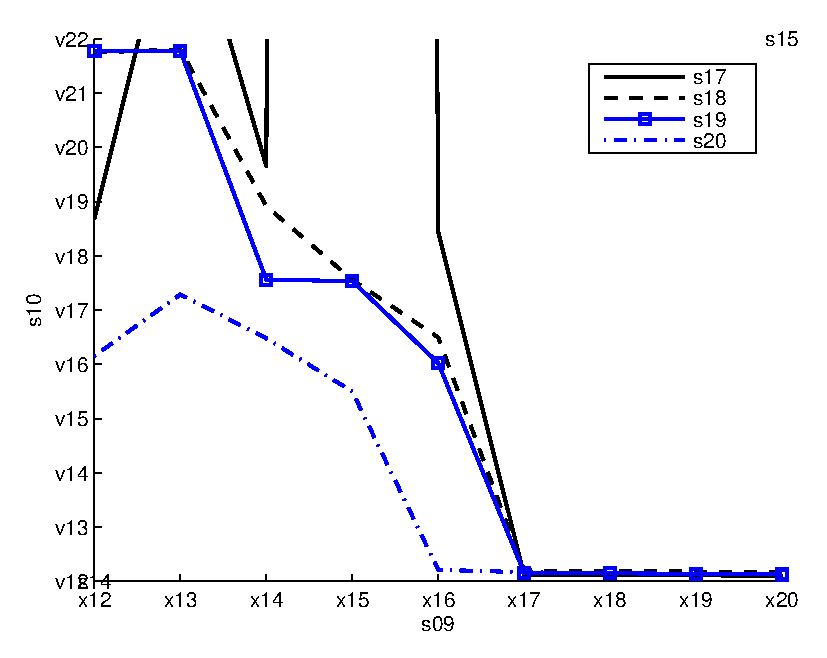
\includegraphics[width=15cm]{mrmse_300.eps}%
\end{psfrags}%
%
% End mrmse_300.tex

\caption{SOC error for $T_s=300$~s as a function of number of integration steps $M$.}
\label{fig:mrmse_300}
\end{figure}

\begin{figure}
\centering
% generated by laprint.m
%
%
% text strings:
\psfrag{s05}[b][b]{\color[rgb]{0,0,0}\setlength{\tabcolsep}{0pt}\begin{tabular}{c}RMSE\end{tabular}}%
\psfrag{s06}[t][t]{\color[rgb]{0,0,0}\setlength{\tabcolsep}{0pt}\begin{tabular}{c}$k$\end{tabular}}%
\psfrag{s10}[][]{\color[rgb]{0,0,0}\setlength{\tabcolsep}{0pt}\begin{tabular}{c} \end{tabular}}%
\psfrag{s11}[][]{\color[rgb]{0,0,0}\setlength{\tabcolsep}{0pt}\begin{tabular}{c} \end{tabular}}%
\psfrag{s12}[l][l]{\color[rgb]{0,0,0}SLF}%
\psfrag{s13}[l][l]{\color[rgb]{0,0,0}EKF}%
\psfrag{s14}[l][l]{\color[rgb]{0,0,0}UKF}%
\psfrag{s15}[l][l]{\color[rgb]{0,0,0}CKF3}%
\psfrag{s16}[l][l]{\color[rgb]{0,0,0}CKF5}%
\psfrag{s17}[l][l]{\color[rgb]{0,0,0}SLF}%
%
% xticklabels:
\psfrag{x01}[t][t]{0}%
\psfrag{x02}[t][t]{50}%
\psfrag{x03}[t][t]{100}%
\psfrag{x04}[t][t]{150}%
\psfrag{x05}[t][t]{200}%
\psfrag{x06}[t][t]{250}%
\psfrag{x07}[t][t]{300}%
\psfrag{x08}[t][t]{350}%
%
% yticklabels:
\psfrag{v01}[r][r]{0}%
\psfrag{v02}[r][r]{0.005}%
\psfrag{v03}[r][r]{0.01}%
\psfrag{v04}[r][r]{0.015}%
\psfrag{v05}[r][r]{0.02}%
\psfrag{v06}[r][r]{0.025}%
\psfrag{v07}[r][r]{0.03}%
\psfrag{v08}[r][r]{0.035}%
%
% Figure:
%
% End rmse_300_64.tex

\caption{RMSE of SOC estimation for $T_s=300$~s and $M=64$.}
\label{fig:rmse_300_64}
\end{figure}

\begin{figure}
\centering
% generated by laprint.m
%
%
% text strings:
\psfrag{s05}[b][b]{\color[rgb]{0,0,0}\setlength{\tabcolsep}{0pt}\begin{tabular}{c}RMSE\end{tabular}}%
\psfrag{s06}[t][t]{\color[rgb]{0,0,0}\setlength{\tabcolsep}{0pt}\begin{tabular}{c}$k$\end{tabular}}%
\psfrag{s10}[][]{\color[rgb]{0,0,0}\setlength{\tabcolsep}{0pt}\begin{tabular}{c} \end{tabular}}%
\psfrag{s11}[][]{\color[rgb]{0,0,0}\setlength{\tabcolsep}{0pt}\begin{tabular}{c} \end{tabular}}%
\psfrag{s12}[l][l]{\color[rgb]{0,0,0}SLF}%
\psfrag{s13}[l][l]{\color[rgb]{0,0,0}EKF}%
\psfrag{s14}[l][l]{\color[rgb]{0,0,0}UKF}%
\psfrag{s15}[l][l]{\color[rgb]{0,0,0}CKF3}%
\psfrag{s16}[l][l]{\color[rgb]{0,0,0}CKF5}%
\psfrag{s17}[l][l]{\color[rgb]{0,0,0}SLF}%
%
% xticklabels:
\psfrag{x01}[t][t]{0}%
\psfrag{x02}[t][t]{50}%
\psfrag{x03}[t][t]{100}%
\psfrag{x04}[t][t]{150}%
\psfrag{x05}[t][t]{200}%
\psfrag{x06}[t][t]{250}%
\psfrag{x07}[t][t]{300}%
\psfrag{x08}[t][t]{350}%
%
% yticklabels:
\psfrag{v01}[r][r]{0}%
\psfrag{v02}[r][r]{0.005}%
\psfrag{v03}[r][r]{0.01}%
\psfrag{v04}[r][r]{0.015}%
\psfrag{v05}[r][r]{0.02}%
\psfrag{v06}[r][r]{0.025}%
\psfrag{v07}[r][r]{0.03}%
%
% Figure:
%
% End rmse_300_256.tex

\caption{RMSE of SOC estimation for $T_s=300$~s and $M=256$.}
\label{fig:rmse_300_256}
\end{figure}

\end{document}
